\usepackage{lipsum}

\begin{document}

% =======================================================================================
%\cleardoublepage % Forces the first chapter to start on an odd page so it's on the right

% =======================================================================================
%                                   PREAMBLE
% =======================================================================================
\coverpage{\TITLE}{\SUBTITLE}{\AUTHOR}{\DATE}{\SUBJECT}
%----------------------------------------------------------------------------------------

\newpage

\paragraph{Abstract}

One of the growing areas of computational intelligence is automatic programming, where a learning algorithm produces executable software. This paradigm promises efficient and highly capable artificial intelligence agents that express their knowledge and reasoning process in a programming language that can be understood, audited and edited by humans, as well as other automated tools - essential requirements for decision support systems in safety-critical application areas such as healthcare.

Of particular interest for healthcare is Programmatically Interpretable Reinforcement Learning, in which a program induction algorithm is used to search for a protocol that performs well in a predictive patient simulator.
The simulator can be derived from clinical data, implemented based on expert knowledge or combine both methods.
Deployment of this approach in real world settings is hindered by the lack of specialized patient simulators and insufficient capabilities of modern program synthesis algorithms.
This work makes contributions to both fields.

The contributions to synthesis algorithms are a novel programming language for general purpose neural program synthesis, a neurogenetic programming framework for program synthesis in BF++ or similar simple languages, a tree variational autoencoder model for code and, finally, Synthesize Execute Debug and Rank: a state-of-the-art iterative algorithm for fully autonomous programming with large language models.

In the field of patient simulators, an anthropodidactic Reinforcement Learning environment for emergency care (Auto-ALS) is introduced, a framework for image-based sonography simulators and a benchmark dataset for intensive care simulation. 

The proposed program synthesis algorithms are evaluated on standard benchmarks as well as Auto-ALS to identify healthcare-specific insights.
The advances introduced in this work lay the foundations for the nascent field of Programmatically Interpretable Reinforcement Learning for Healthcare.

\tableofcontents

\addcontentsline{toc}{section}{List of Figures}
\listoffigures

\addcontentsline{toc}{section}{List of Tables}
\listoftables

\addcontentsline{toc}{section}{Nomenclature}
\nomenclature{PBE}{Programming by example \cite{gulwani2016:programming, halbertProgrammingExample1984}}
\nomenclature{PIRL}{Programmatically Interpretable Reinforcement Learning \cite{pirl}}
\nomenclature{PatientSPIRL}{Patient Simulator Programmatically Interpretable Reinforcement Learning, introduced in chapter \ref{ch:proposal}}

\nomenclature{RL}{Reinforcement Learning \cite{suttonReinforcementLearningSecond2018}}
\nomenclature{PQT}{Priority Queue Training \cite{abolafiaNeuralProgramSynthesis2018}}
\nomenclature{POMDP}{Partially Observable Markov Decision Process \cite{kramerjdavidrPartiallyObservableMarkov1964}}
\nomenclature{MPC}{Model Predictive Control \cite{garciaModelPredictiveControl1989, holkarOverviewModelPredictive2010, kouvaritakisModelPredictiveControl2016, schwenzerReviewModelPredictive2021}}
\nomenclature{MDPD}{Message Passing Decision Process, introduced in section \ref{sec:mpdp}}

\nomenclature{GPT}{Generative Pre-trained Transformer \cite{radfordImprovingLanguageUnderstandinga}}
\nomenclature{LLM}{Large Language Model}
\nomenclature{AI}{Artificial Intelligence}

\nomenclature{CASE}{Computer-Aided Software Engineering \cite{ComputeraidedSoftwareEngineering2025}}
\nomenclature{AST}{Abstract Syntax Tree, see \ref{sec:grammar-guided}}

\nomenclature{SEIDR}{Synthesize Execute Debug Rank, introduced in chapter \ref{ch:seidr}}

\nomenclature{MHE}{Moving Horizon Estimator}

\nomenclature{CAPFT}{Capacity modifier function with temperature}
\nomenclature{CO2}{Carbon dioxide}
\nomenclature{EIR}{Energy input ratio}
\nomenclature{EIRFT}{Energy input ratio function with temperature}
\nomenclature{EIRFPLR}{Energy input ratio function with partial load ratio}
\nomenclature{HVAC}{Heating Ventilation Air Conditioning}
\nomenclature{IDEAS}{Integrated District Energy Assessment Simulations}
\nomenclature{IPOPT}{Interior Point Optimizer}
\nomenclature{KPI}{Key Performance Indicator}
\nomenclature{PI}{Proportional Integral}
\nomenclature{PLR}{Partial load ratio}
\nomenclature{RC}{Resistance capacitance}

\nomenclature{ALS}{Advanced Life Support \cite{AMLSAdvancedMedical2021}}

\newcommand{\obs}{\mathbf{o}}
\nomenclature{$\obs$}{a single observation of an agent}

\newcommand{\policy}{\pi}
\nomenclature{$\policy(\action)$}{a \emph{policy distribution} that stochastically defines the agent's actions}
\nomenclature{$\policy(\text{text})$}{language model (probability distribution over texts)}

\newcommand{\discretebins}{\Upsilon^\text{bins}}
\nomenclature{$\discretebins$}{number of discretization bins}

\newcommand{\historylen}{\Upsilon^\text{history}}
\nomenclature{$\historylen$}{history length, the number of past steps considered by the algorithm}

\newcommand{\mlinput}{x}
\newcommand{\mlinputvec}{\mathbf{x}}
\nomenclature{$\mlinput$, $\mlinputvec$}{input examples in a machine learning system}

\newcommand{\step}{i}
\newcommand{\stepp}{j}
\newcommand{\steppp}{k}
\nomenclature{$\step$,$\stepp$,$\steppp$}{iteration, step, moment in discrete time}

\newcommand{\mloutput}{y}
\newcommand{\mloutputvec}{\mathbf{y}}
\nomenclature{$\mloutput$, $\mloutputvec$}{expected output examples in a machine learning system}

\newcommand{\obss}{\mathcal{O}}
\nomenclature{$\obss$}{set of all possible observations $\obs$}

\newcommand{\state}{\textbf{s}}
\nomenclature{$\state$}{a state of an environment}

\newcommand{\states}{\mathcal{S}}
\nomenclature{$\states$}{set of all possible states $\state$ of an environment}

\newcommand{\termstates}{\mathcal{S}_t}
\nomenclature{$\termstates$}{set of all terminal states $\state$ of an environment}

\newcommand{\nontermstates}{\mathcal{S}_{nt}}
\nomenclature{$\nontermstates$}{set of all non-terminal states $\state$ of an environment}

\newcommand{\action}{a}
\nomenclature{$\action$}{an action of an agent}

\newcommand{\actions}{\mathcal{A}}
\nomenclature{$\actions$}{set of all possible actions $\action$}

\newcommand{\actionqueue}{\alpha}
\nomenclature{$\actionqueue$}{action queue of an agent}

\newcommand{\reward}{r}
\nomenclature{$\reward$}{a reward}

\newcommand{\returnn}{R_n}
\nomenclature{$\returnn$}{n-step return}

\newcommand{\returntot}{R_\text{tot}}
\nomenclature{$\returntot$}{total episode return}

\newcommand{\realnums}{\mathbb{R}}
\nomenclature{$\realnums$}{real numbers}

\newcommand{\memory}{m}
\nomenclature{$\memory$}{memory of an agent}

\newcommand{\alphabet}{\aleph}
\nomenclature{$\alphabet$}{the alphabet of a programming language (set of all possible tokens $\token$)}

\newcommand{\token}{c}
\nomenclature{$\token$}{a \emph{token}, a minimal unit of code, such as a character}

\newcommand{\code}{\mathcal{C}}
\nomenclature{$\code$}{\emph{program code}, a sequence of tokens $\token_1,\token_2,\dots$ that constitutes a program}

\newcommand{\codebase}{\kappa}
\nomenclature{$\codebase$}{\emph{codebase}, a population of programs}

\newcommand{\expectation}{\mathbb{E}}
\nomenclature{$\expectation$}{expected value}

\newcommand{\loss}{\lambda}
\nomenclature{$\loss(x)$}{a differentiable loss function to be minimized by an optimization algorithm}

\newcommand{\obj}{\omega}
\nomenclature{$\obj(x)$}{an objective function to be maximized by an optimization algorithm}

\newcommand{\learnables}{\Phi}
\nomenclature{$\learnables$}{learnable parameters of a model}

\newcommand{\weights}{\mathbf{W}}
\nomenclature{$\weights$}{weight matrix in a model, element of $\learnables$}

\newcommand{\biases}{\mathbf{b}}
\nomenclature{$\biases$}{bias vector in a model, element of $\learnables$}

\newcommand{\hidden}{\mathbf{h}}
\nomenclature{$\hidden$}{a hidden state within a model}

\newcommand{\latent}{\mathbf{z}}
\nomenclature{$\latent$}{a latent representation of input $\mlinput$}

\newcommand{\mean}{\boldsymbol\mu}
\nomenclature{$\mean$}{mean}

\newcommand{\stddev}{\boldsymbol\sigma}
\nomenclature{$\stddev$}{variance}

\newcommand{\normaldistr}{\nu}
\nomenclature{$\normaldistr(\mean,\stddev)$}{the normal distribution}

\newcommand{\pointer}{P}
\nomenclature{$\pointer$}{pointer}

\newcommand{\prob}{p}
\nomenclature{$\prob(x)$}{a probability distribution}

\newcommand{\team}{\Xi}
\nomenclature{$\team$}{a cooperative \emph{team} of agents}

\newcommand{\temp}{T}
\nomenclature{$\temp$}{sampling temperature}
\nomenclature{$\temp$}{physical temperature}

\newcommand{\timepoint}{t}
\nomenclature{$\timepoint$}{a moment in continuous time}

\newcommand{\threshold}{\theta}
\nomenclature{$\threshold$}{threshold value for discretization}

\newcommand{\hyperparam}{\Upsilon}
\nomenclature{$\Upsilon$}{hyperparameter of an algorithm}

\newcommand{\beamwidth}[0]{\hyperparam^\text{beam}}
\nomenclature{$\beamwidth$}{beam width in beam search}

\newcommand{\treearity}[0]{\hyperparam^\text{tree}}
\nomenclature{$\treearity$}{tree arity, as in $\treearity$-ary tree}

\newcommand{\integers}{\mathbb{Z}}
\nomenclature{$\integers$}{integers}

\newcommand{\treenode}{\delta}
\nomenclature{$\treenode$}{a node in a tree}

\newcommand{\kldivergence}{D_{KL}}
\nomenclature{$\kldivergence(\prob_L \parallel \prob_R)$}{Kullback Leibner divergence between probability distributions $\prob_L(x)$ and $\prob_R(x)$, $\sum_x \prob_L(x)\ \log\left(\frac{\ \prob_L(x)\ }{ \prob_R(x) }\right)$}

\newcommand{\identitymatrix}{I}
\nomenclature{$\identitymatrix$}{identity matrix}

\newcommand{\regularization}{\hyperparam^\text{regularization}}
\nomenclature{$\regularization$}{weight of a regularization term in $\obj(x)$}

\newcommand{\greed}{\hyperparam^\text{greed}}
\nomenclature{$\greed$}{greed level setting for a greedy algorithm}

\newcommand{\probs}{\mathcal{P}}
\nomenclature{$\probs$}{a set or tuple of probability distributions}

\newcommand{\statevalue}{V}
\nomenclature{$\statevalue(\state)$}{value of a state in reinforcement learning}

\printnomenclature

\emph{A note on notation:} bold lowercase characters $\mathbf{x}$ represent vectors, bold uppercase characters $X$ represent matrices, calligraphic letters $\mathcal{X}$ represent sets and tuples. This holds for functions as well, i.e. $f(\mathbf{x})$ maps vectors to scalars
\printnomenclature

% =======================================================================================
%                                   PART I
% =======================================================================================
\part{Program Induction}
%----------------------------------------------------------------------------------------
\newpage
\chapter{The Promise} \label{ch:autocode-motiv}
\section{The Quest of Automatic Programming \cite{liventsevTaxonomyAutomaticProgramming2023}}
\label{sec:quest}

\emph{Automatic programming} or \emph{program synthesis} refers to any technological setup wherein the task of writing computer programs is automated. 
First introduced in science fiction \cite{jenkinsLogicNamedJoe1946}, it is now an active area of technical research.
Program synthesis systems are defined by what type of task \emph{specification} they admit, whether and how the generated programs are verified, whether and how pre-existing programs are incorporated \cite{gulwaniDimensionsProgramSynthesis2010}.

\begin{figure}[H]
    \centering
    \includegraphics[width=\linewidth]{ap.png}
    \caption{Automatic programming system, schematic definition}
    \label{fig:ap}
\end{figure}

This definition is purposefully broad and includes, for example, the compiler \cite{penjamDeductiveInductiveMethods2003,patrickmckenzie[@patio11]GlibLineHave2023}: a program synthesis system that admits a specification in the form of a program in a high-level programming language designed for ease of use by humans and generates a program in a low-level programming language designed for ease of deployment on a computer.

\begin{figure}[H]
    \centering
    \includegraphics[width=\linewidth]{compiler.png}
    \caption{Compiler, schematic definition}
    \label{fig:compiler}
\end{figure}


The ambition of the field, however, extends far beyond compilers \cite{campbellAutomatedCodingQuest2020}.
The goal is to impose as few constraints as possible onto the \emph{specification} and ultimately automate the generation of programs for any free-form specification, such as a short textual \cite{zanLargeLanguageModels2023} prompt or a diagram \cite{koziolekLLMbasedControlCode2023}, even a hand-drawn sketch \cite{chatgptmodderChatgptCanNow2023}.

% TODO: examples for the above

\newpage
\section{Taxonomy of tasks \cite{liventsevTaxonomyAutomaticProgramming2023}}
\label{sec:taxonomy}

\paragraph{Code translation}

The humble compiler from section \ref{sec:quest} is an instance of a \emph{code translation} system: a \emph{program synthesis} system where the specification is given as text, either in a natural language (\emph{NL2Code translation} \cite{wangNaturalLanguageCode2023, zanLargeLanguageModels2023}) or in a programming language (\emph{code2code translation} \cite{radfordImprovingLanguageUnderstanding})
Code to natural language translation is studied as well \cite[section 5.1]{leDeepLearningSource2020}, but it is less common and out-of-scope for this work.
Intelligent conversational assistants (\href{https://chat.openai.com/}{ChatGPT}, \href{https://gemini.google.com}{Gemini}, \href{https://claude.ai/}{Claude}, \href{https://pi.ai/}{Pi}) with program synthesis functionality operate in the translation paradigm as they translate a text specification into code.

\begin{figure}[H]
    \centering
    \includegraphics[width=\linewidth]{nl2ml.png}
    \caption{Code translation, schematic definition}
    \label{fig:nl2ml}
\end{figure}

\paragraph{Programming by example}

Another approach to specification is specifying the expected output of the program. Or, since in most interesting programs the output depends on the input, \emph{input-output pairs}. This task is known as \emph{programming by example} \cite{halbertProgrammingExample1984, psb2}.

\begin{figure}[H]
    \centering
    \includegraphics[width=\linewidth]{pbe.png}
    \caption{Programming by example, schematic definition}
    \label{fig:pbe}
\end{figure}

The goal of a programming by example system is to find a program $f$ such that $\outputvec=f(\inputvec)$ for a given vector of input-output pairs $(\inputvec,\outputvec)$. 
Note that this is exactly the definition of \emph{supervised learning}~\cite{cunninghamSupervisedLearning2008}.
Indeed, \emph{programming by example} is an unusual type of \emph{supervised learning}, one where the trained model is expressed as source code.

The prime application of \emph{programming by example} is \emph{data wrangling} tools such as Microsoft Excel \cite{gulwaniProgrammingExamplesandIts2016} where it is used as a data extrapolation tool: if a formula $f$ can be synthesized that satisfies $\outputvec=f(\inputvec)$, one can generate $\outputvec '=f(\inputvec ')$ for future values $\inputvec '$.
\emph{Programming by example} is also used in scientific domains to generate formulas that fit experimental observations, where it is known as \emph{symbolic regression} \cite{makkeInterpretableScientificDiscovery2022}.

\paragraph{PIRL}

Not every task, however, can be easily described with input-output examples. 
Take chess: it's relatively simple to evaluate the performance of a chess-playing program, but what are the \emph{correct} moves? 
That is simply not known in advance.
Given enough trial and error it's still possible to generate a correct program with such black box specification, a task known as \emph{Programmatically Interpretable Reinforcement Learning} \cite{pirl}.

\begin{figure}[H]
    \centering
    \includegraphics[width=\linewidth]{pirl.png}
    \caption{Programmatically Interpretable Reinforcement Learning, schematic definition}
    \label{fig:pirl}
\end{figure}

In this setting, a program gets generated and deployed in an environment that responds with positive and negative rewards. 
The most common formalism for such an environment as Partially Observable Markov Decision Process \cite{kramerjdavidrPartiallyObservableMarkov1964, spaanPartiallyObservableMarkov2012}: when at step $i$ the agent takes action $a_i \in \rlactionspace$ it has an impact on  the state of the environment $s_i \in \rlstatespace$ via distribution $\rlstatedistr$ of conditional probabilities of possible subsequent states. 
State is a latent variable that the agent cannot observe.
Instead, the agent can see an observation $o_i \in \rlobsspace$ which is a random variable that depends on the latent state via distribution $\rlobsdistr$.
$\rlactionspace$, $\rlstatespace$ and $\rlobsspace$ are sets of all possible actions, states and observations respectively.
Finally, at every step the agent observes a reward $\rlrewardf$

Given this limited toolset, without full (or any) prior knowledge of how the agent's actions influence the the environment (distributions $\rlstatedistr$ and $\rlobsdistr$), the agent has to come up with a strategy that will maximize $n$-step return $R_n=\sum_{t=i}^{n} r_t$ where $n$ is the agent's planning horizon. It is, in the general sense, a hyperparameter, however if an environment has a limit on how many steps an episode can last, it is reasonable to set $n$ equal to the step limit. 

\newpage
\section{Why not just use Machine Learning?}

As programmatically interpretable cousins of \emph{supervised learning} and \emph{reinforcement learning} respectively, \emph{Programming by example} and \emph{PIRL} are  used in settings where more traditional machine learning methods that don't involve code generation could also be used.
What are then the advantages conferred by this programmatic representation?

\paragraph{Expressiveness and performance}

Programming languages benefit from decades of research dedicated to making them \textcolor{accent}{expressive} - able to efficiently represent any algorithm one can design - and \textcolor{accent}{performant} - making those algorithms executable with minimal requirements of time and hardware.
Machine learning models don't have this advantage - they are designed to make the space of possible models easy to search and optimize in, often at the expense of expressivity and performance: an equivalent program typically solves the task better and faster than a machine learning model, to the point where representing algorithms as neural networks has become a setup of programmer humor \cite{JoelGrusFizz}.

In fact, \cite{JoelGrusFizz} underestimates the inefficiency of the neural network approach, since in their neural network implementation of FizzBuzz algorithm an important part (output of text) is non-neural.
We correct for this and train\footnote{\url{github.com/vadim0x60/fizzbuzzlm}} a specialized language model for FizzBuzz, \emph{FizzBuzzLM}, benchmarking it against implementations of the same algorithm in major programming languages.

\begin{table}[H]
    \centering
    \begin{tabular}{r|r|l}
         Language & source, bytes & CPU runtime \\
         \midrule
         C & 321 & 340.3 µs ± 117.0 µs \\
         Clojure & 178 & 507.2 ms ± 6.5 ms \\
         C\# & 289 & 60.4 ms ± 4.8 ms \\
         Go & 295 & 966.5 µs ±  93.2 µs \\
         Haskell & 213 & 16.1 ms ± 0.4 ms \\
         Java & 403 & 28.9 ms ± 0.6 ms \\
         JavaScript & 162 & 30.1 ms ± 0.4 ms \\
         Python & 192 & 44.9 ms ± 0.6 ms \\
         Rust & 307 & 573.5 µs ± 114.3 µs \\
         FizzBuzzLM & 13177 & 853.2 ms ± 6.8 ms\footnote{GPU (NeuralEngine) runtime was even slower, at 1.596 s ± 0.037 s}
    \end{tabular}
    \caption{Performance charecteristics of different FizzBuzz implementations}
    \label{tab:my_label}
\end{table}

We can see that the programming language implementations are somewhat faster than \emph{FizzBuzzLM} and much more expressive with at least \emph{FizzBuzzLM} 2 orders of magnitude behind the true Kolmogorov complexity \cite{kolmogorov} of th3e problem.
The only reason why these performance costs are accepted is that it's easier to implement optimization in the space of possible neural network parameters than in the space of possible programs. 
When the problem of optimal program synthesis is solved, it becomes the "best of both worlds" approach: data-driven and trainable, but using an expressive an performant representation.
 
\paragraph{Import and export of knowledge}

Programs as a representation for decision-making of a model have a chance to become the \emph{lingua franca} \cite{samarinLinguaFranca1987} for representing decision processes as they can be understood both by a wide variety of machine learning/artificial intelligence systems and by humans, enabling humans and robots trying to tackle the same problem to learn from each other.

\begin{figure}[H]
    \centering
    \includegraphics[width=\linewidth]{mlvsautocode.png}
    \caption{Program synthesis allows for knowledge sharing}
    \label{fig:mlvsautocode}
\end{figure}

The search in a space of possible programmatic solutions to a problem can be initialized with an existing program that has been developed by an expert in the field (perhaps with the  use of AI tools), thus \textcolor{accent}{importing existing knowledge} from previous efforts of solving the same problem.
This process is not dissimilar to what is known in deep learning as \emph{fine-tuning}: initializing the optimization process of model parameters with a model already trained on a similar task, but it has the additional advantage that the initial code can be generated by a model of a completely different architecture or by a human.

After the search process has been concluded, all of the knowledge incorporated into the resulting system can be \textcolor{accent}{examined and verified}. 
Unlike the black-box model, the approach makes it trivial to answer questions like "Does this model include factor X in its decision-making on topic Y?".
This offers us an additional way of verifying the decision system before its final deployment. 
And, unlike the numerous post-hoc methods of machine learning interpretability \cite{linardatosExplainableAiReview2020}, this approach involves a strong guarantee that the explanation does not diverge from the behavior.

Of course, the external observers of a program synthesis system can be not only teachers, but also students. 
Even if the resulting program is never deployed, one can read it and \textcolor{accent}{export the knowledge} and incorporate it into future systems, as well as textbooks and other didactic materials for humans.

\newpage
\section{Broader impacts}

\epigraph{The Future's So Bright, \\ I Gotta Wear Shades}{Timbuk 3}

\paragraph{Capability}

The \emph{expressivity and peformance} of programming languages can lead to \emph{decision support systems}, also known as \emph{digital assistants}, that are more capable, better able to make predictions and provide advice.

The ability to \emph{import, verify and export knowledge} into or out of a decision suport system can reduce or even eliminate the amount of \emph{knowledge silos} that exists in the ecosystem of these agents, where each separate system has been trained on some data set of its own and some expert knowledge of its own and each incorporates some small part of existing knowledge about the field. 

Insufficient capability in digital assistants can be a major safety risk, especially when they're deployed fully autonomously. For example, misidentification of obstacles in autonomous driving \cite{sheebajoiceObstacleDetectionSafe2023} or wrongful diagnosis in healthcare \cite{wintersDiagnosticErrorsIntensive2012} can be a matter of life and death.

\paragraph{Alignment}

Highly capable digital assistants present their own family of safety risks. 
If perverse incentives are present in the optimization goals of the decision system, then a highly capable decision system can bring about harmful situations intentionally.
Most optimization targets are imperfect proxies of intended outcomes. 
An optimization process can thus \emph{game} (\emph{hack}) the metrics and achieve negative outcomes, despite technically improving the metrics.
Common types of \emph{reward hacking} \cite{skalseDefiningCharacterizingReward2022} include:
\begin{description}
    \item[reward tampering] \cite{everittRewardTamperingProblems2021, skalseInvariancePolicyOptimisation2023} - acting on the reward mechanism directly, i.e. disabling sensors involved in performance evaluation or writing more flattering documentation.
    \item[adverse selection] - selectively solving subtasks that are easier to solve even if they happen to be more important.
\end{description}

To give a real world example, both phenomenons have been observed in Healthcare: \cite{shenSelectionIncentivesPerformance2003} find that incentives can lead to the most severely ill patients being less likely to receive care. \cite{fairbrotherImpactFinancialIncentives2001, ImpactPhysicianBonuses, roskiImpactFinancialIncentives2003} find that metrics are sometimes improved by better documenting the incentivized results, not improving them.
\cite{longFairnessMachineLearning2021} notes how misguided fairness metrics incentivize decision systems to intentionally harm people from healthier demographic groups in order to advance equality of outcomes ("equity").

These issues are present in society \cite{nestianPerverseIncentiveGeneral2017} with or without artificial intelligence, they are studied in economics under the umbrella of the \emph{principal agent problem} \cite{pandaAgencyTheoryReview2017}. 
However, powerful optimization algorithms have potential to exacerbate those issues \cite{hadfield-menellIncompleteContractingAI2019}. 
And while the first line of defense is, of course, improving the incentives, one can be skeptical as to whether the incentives can ever represent their designers' intentions perfectly.

In fact, the instrumental convergence theory \cite{benson-tilsenFormalizingConvergentInstrumental} posits that perverse incentives are inherent to any reinforcement learning context, because optimizing for any goal can be aided by increasing the amount of control over one's environment the agent has, and thus any optimization of agents creates incentives to maximize their own power and control. 
First introduced in science fiction \cite{clarke2001SpaceOdyssey2016, ellisonHaveNoMouth1967, jonesColossus2019}, this is now an active area of technical research \cite{jiAIAlignmentComprehensive2024}.
Estimates of the potential dangers of misaligned artificial intelligence range from non-trivial to existential \cite{mcleanRisksAssociatedArtificial2023}.

The interpretability afforded by the program synthesis approach provides a second line of defense against perverse incentives, namely examining the control program and trying to establish whether any of the modules in that program are attempting to game the optimization metrics, manually or with the use of AI tools.

\begin{figure}[H]
    \centering
    \includegraphics{PSAlign.drawio}
    \caption{Program Synthesis as an alignment methodology}
    \label{fig:ps-as-alignment}
\end{figure}

As the field of artificial intelligence advances, this advances both the generative tools and the verification tools, thus making program synthesis a viable approach to scalable oversight \cite[section 5]{amodeiConcreteProblemsAI2016}.

\paragraph{Human-Robot Teams}

Transparency is a foremost principle of effective teamwork: every member of the team is supposed to know what and why every other member is doing. 
This principle is supported by the study of human teams \cite{bagPEERTRANSPARENCYTEAMS2012a, solomonInferenceTransparencyEffective2021b} and human-robot teams \cite{ezenyilimbaImpactTransparencyExplanations2022, guznovRobotTransparencyTeam2019, holderDesigningBiDirectionalTransparency2021, lakhmaniExploringEffectCommunication2019, lakhmaniProposedApproachDetermining2016, mercadoIntelligentAgentTransparency2016, ososkyDeterminantsSystemTransparency2014, Panganiban2019Transparency, ronconeTransparentRoleAssignment2017} alike.
Some literature in Human-Robot teams takes inspiration \cite{shivelyCrewResourceManagement2018} from teamwork research in aviation where studies into the common causes of incidents and accidents \cite{chidesterPersonalityFactorsFlight1990, chidesterPilotPersonalityCrew1991, smithSimulatorStudyInteraction1979} have been used to formulate core principles of Crew Resource Management, such as "Verbalize Verify Monitor".
And as more automation is introduced in aviation, the modern cockpit itself can be seen as a human robot team.
Same is true of an operating theater with a robot assistant \cite{weerarathnaHumanRobotCollaborationHealthcare2023} or a doctor using a clinical decision support system \cite{castilloConsiderationsSuccessfulClinical2013, mooreIntroductionClinicalDecision2011, osullivanDecisionTimeClinical2014, purcellWhatMakesGood2005, sakallarisClinicalDecisionSupport2000, selfClinicalDecisionSupport2008, stangeThisIssueClinical2011, wrightClinicalDecisionSupport2009}

The lack of transparency is an important roadblock for integration of black box decision systems in safety critical domains: when conflict arises between the opinion of the expert and the opinion of the system, a black box system offers no additional information for the resolution of the conflict. 
A program, on the other hand, offers the experts a way to explicitly examine why a certain advice is given and use this information to take or not take the advice into account. 
Consequently, a black box system can only be used to completely replace a certain job - any setting where a collaboration is required between a human and decision system requires some degree of transparency that can be afforded by technology like program synthesis. 
This ensures synergistic decision-making where the analysis of every participant is taken into account of the final decision.

\paragraph{Compliance}

Both individual organizations and regulatory authorities often impose requirements onto their decision systems that assume their transparency. 
An audit has to be able to establish whether the system displays any illegal patterns such as a violation of established clinical protocol in healthcare or unauthorized discrimination in insurance and lending. 
Such requirements have had a chilling effect on the real world deployment of deep learning systems. 
A program, on the other hand, can be audited and proven to be compliant. 
Program synthesis can thus bring all the advantages of big data-driven systems into such fields without necessitating a regulatory reform.

\paragraph{Privacy}

The ineffiency of inference of current machine learning models is (along with competitive pressures) a core reason of the "cloudification" of artificial intelligence: as of late 2023, the most powerful products of machine learning \cite{achiamGpt4TechnicalReport2023} are distributed as remote services that can be interacted with, but not fully copied, via the Internet.
Asking a state of the art decision support system for advice means sending the (potentially sensitive) request to the model provider and making both requests and responses known to said provider \cite{PrivacyPolicy}.
Programs, in contrast, are easier to distribute and performant enough to run on most devices most of the time.
The advent of program synthesis can pave the way to more privacy-preserving decision support: even if the generative model remains in the cloud, one can first use the model to synthesize the program, download it and then submit the sensitive data to the program locally.

% Add a point about IP

\paragraph{Scientific discovery}

Lastly, export of knowledge out of a automatic programming system can be a powerful tool of scientific discovery. 
Symbolic regression is already widely used in physics in order to find formulas that fit experimental results \cite{angelisArtificialIntelligencePhysical2023, tenachiDeepSymbolicRegression2023}. 
In fact, it is not unreasonable to claim that physics \emph{is} a set of symbolic regression problems \cite{udrescuAIFeynmanPhysicsinspired2020}, historically solved manually, but increasingly with some application of algorithms. 
The same can be said about biology \cite{chenRevealingComplexEcological2019}, economics \cite{claveriaAssessmentEffectFinancial2017, lianModelingForecastingPassenger2018, panInfluentialFactorsCarbon2019, truscottDetectingShadowEconomy2011, truscottExplainingUnemploymentRates2014, yamashitaCustomizedPredictionAttendance2022} or any field that develops formulas based on series of empirical observations.

%----------------------------------------------------------------------------------------
\newpage
\chapter{The State of the Art}\label{ch:autocode-sota}
Automatic program synthesis has been a long term goal of the field of artificial intelligence since its inception \cite{mannaAutomaticProgramSynthesis1971}, promising to reduce the workload of software developers by automatically solving some of the tasks they face.
And since the field's inception it has been grappling with the challenging properties of the sparse optimization space \cite{alurSyntaxguidedSynthesis2013, davidProgramSynthesisChallenges2017} that is the set of all programs in a certain programming language, namely, 
\begin{enumerate}
    \item valid error-free programs constitute an exceedingly small part of the space of possible strings, so any program synthesis algorithm that incorporates random guessing (for instance, Reinforcement Learning with random initialization \cite{suttonReinforcementLearningSecond2018}) is exceedingly unlikely to guess a valid program;
    \item a small edit in a program can result in a large difference in it's behavior (and, conversely, the same algorithm can be expressed with very different programs), hence the programs we would like to find are not clustered in any compact part of the optimization space;
    \item some of the evaluation mechanisms of programs, especially in the \emph{Programmatically Interpretable Reinforcement Learning} paradigm involve stochasticity and can yield different results for the same program.
\end{enumerate}

In other words, the search space in program synthesis is \emph{sparse}, \emph{brittle} and sometimes \emph{noisy} \cite{arnoldNoisyOptimizationEvolution2002} - all known challenges in Optimization Theory.

\newpage
\section{Genetic programming}

\begin{figure}[H]
    \centering
    \includegraphics[width=\linewidth]{gp.png}
    \caption{Genetic Programming, schematic definition}
    \label{fig:gp}
\end{figure}

The family of optimization methods best applicable to this type of complex non-differentiable search space is \emph{genetic and evolutionary methods} - biologically inspired methods that operate on a population of candidate solutions (programs), randomly edit (\emph{mutation}) and combine (\emph{recombination}) to expand the population and the prune the population by \emph{natural selection}: removing the candidates that adhere to the specification the least.
Within program synthesis this family of methods is known as \emph{genetic programming} \cite{genprog1, genprog2, genprogast}
In an evolutionary setting, as soon as at least one (preferably several) valid program is found, initializing the population to include them drastically speeds up the search process, thus addressing the sparsity issue.
This approach is particularly powerful in a setting where some solutions are already known, but a program synthesis system can be used to search for solutions that fit the \emph{specification} even better, a setting known as \emph{genetic improvement of software} \cite{petke2018:genetic}.

Genetic programming has been successfully applied in various domains, including prediction and control \cite{dracopoulosGeneticProgrammingPrediction1997}, the synthesis of complex structures (Koza, 2003), and the evolution of neural network modules \cite{degarisGENETICPROGRAMMING1990}. In the field of engineering, genetic programming has been applied to systems modeling, control, optimization, scheduling, design, and signal processing \cite{willisGeneticProgrammingIntroduction1997}. 

The biggest drawback of GP is that it requires generation and evaluation of a very high number of programs: higher than most other methods (see chapter \ref{ch:seidr}).
If evaluation of a generated program is computationally expensive, this translates directly into a very high computational cost of program synthesis.

\newpage
\section{Constrained programming languages}

Another way to address the complexity of the search space is to select a programming language such that the space of possible programs in that programming language exhibits less of the undesirable properties of optimization spaces.
For examples, a language where any combination of valid characters is a valid program \cite{brainfuck} eliminates a significant share of the complexity of the problem.
This family of approaches is explored in more detail in chapter \ref{ch:bfpp}, including  introduction of a novel constrained programming language for \emph{programmatically interpretable reinforcement learning}

\paragraph{Domain specific languages}

\cite{fowlerDomainspecificLanguages2010, hudakDomainspecificLanguages1997, karsaiDesignGuidelinesDomain2014, kosarComparingGeneralpurposeDomainspecific2010, kosarDomainspecificLanguagesSystematic2016, mernikWhenHowDevelop2005}

\paragraph{Logic programming}

One domain that's particularly amenable to solving synthesis tasks is logic programming:  a programming paradigm based on formal logic \cite{doetsLogicLogicProgramming1994, lloydFoundationsLogicProgramming2012}. 
In constrast to other programming paradigms \cite{floydParadigmsProgramming2007, gorodniaiaStudyProgrammingParadigms2016, krishnamurthi13ProgrammingParadigms2019, vanroyProgrammingParadigmsDummies2009} 

Instead of (or in addition to) generating a program first and testing whether it adheres to specification, \emph{deductive} methods apply equivalence rules to translate the specification into an executable.
This is hard to apply in \emph{programmatically interpretable reinforcement learning} where the specification is a black box, but can be a powerful approach in \emph{code translation} and \emph{programming by example} paradigms.



\newpage
\section{Pre-training methods}

\emph{Inductive synthesis}

\emph{concept space}

The paradigm of foundation models \cite{foundation-models} has recently been very prominent in machine learning and machine learning on source code is no exception.
In this paradigm, a model is first trained on a large dataset to solve a generic task such as next-token prediction and then used as a central component in solutions of various specific tasks.
The foundation models for source code, based on architectures such as GPT Codex \cite{radfordImprovingLanguageUnderstanding,chenEvaluatingLargeLanguage2021,codegen,gpt-neo} and BERT \cite{devlinBERTPretrainingDeep2019,codebert} have enabled significant process in tasks like programming by example \cite{halbertProgrammingExample1984} and even human-comparable performance in coding competitions \cite{liCompetitionLevelCodeGeneration2022}.

\paragraph{Autoregressive models}


\paragraph{Autoencoder models}

While undoubtedly useful in many program synthesis tasks, popular foundation models may fall short in the areas of genetic programming \cite{genprogast} and genetic improvement of software \cite{petke2018:genetic}.
In this settings, new programs are found by exploring the space of programs similar to one or several reference programs.
The task of applying these perturbations to programs could benefit from a foundational model, however, it's unclear how to achieve this with the current autoregressive models.
Autoencoder Genetic Programming \cite{autoenc-gp,denoising-autoenc-gp,latentspaceopt} argues for using autoencoder \cite{autoencoders} models instead.
These models embed programs into a high-dimensional vector space, making it easy to mutate a program by add random noise to the embedding vector or combine several programs by averaging their embedding vectors.

\newpage
\section{Grammar guided synthesis}

Another way to constrain the hypothesis space is to use the grammar of the programming language in question directly in the program generation process.

Unlike natural languages, programming languages are easier to represent structurally due to the nature of their syntax which improves machine learning performance.

\newpage
\section{Human in the loop}

\paragraph{Completion}

\paragraph{Sketching}

\paragraph{Differentiable programming}

\newpage
\section{Open problems}

Most open problems lie in the domain of \emph{Programmatically Interpretable Reinforcement Learning}

However, a fully autonomous system for Programmatically Interpretable Reinforcement Learning is yet to be devised. In chapter \ref{ch:bfpp}

\newpage
\chapter{BF++: a Novel Language for PIRL}\label{ch:bfpp}
\citeself{chapter}{liventsev2021:bf}

\section{BF++}
\label{sec:language}

\paragraph{BF syntax}
\label{sec:bf}

Abolafia {\sl et al} \cite{abolafiaNeuralProgramSynthesis2018} picked BF\footnote{Brainfuck} \cite{brainfuck} as their language for program synthesis for the following reasons:
\begin{itemize}
    \item In industry-grade programming languages like Python or Java program code can contain a very large variety of characters since any of the 143859 Unicode \cite{allenUnicodeStandard2012} characters can be used in string literals. In BF, however, only 8 characters can be used: they can be one-hot-encoded with vectors of size 8. 
    \item BF's simple syntax means that an arbitrary string of valid characters is likely to be a valid program. 
    In more complex languages, most possible strings result in a syntax error. 
    A generative model being trained to write programs in such a language risks being stuck in a long exploration phase when all the programs it generates are invalid and it has no positive examples in the dataset.
    \item Despite all of the above, it is a Turing-complete language.
\end{itemize}

The simplicity of the language also means that it is relatively easy to develop a compiler that translates programs from an industry-standard programming languages like Java and Python to BF thus making use of the expert knowledge existing in those languages. 

In the current chapter, we introduce an extended version of the original BF language, BF++. As explained below, the extensions to the original BF syntax are particularly useful in the RL use cases. 

BF's runtime model is inspired by the classic Turing Machine \cite{turing}: at any point during the program's execution, the state of the program consists of:

\begin{itemize}
    \item An infinite\footnote{If one happens to be executing a BF program on a computer with finite memory, the tape will be finite due to hardware limitations.} tape of cells $T$ where each cell holds an integer number.
    \item A \textit{memory pointer} $p_T$ that points to a certain cell in the tape (\textit{active cell} $T^{p_T}$).
    \item A string of characters $C$ that represents program code.
    \item A \textit{code pointer} $p_C$ pointing to a character about to be executed.
\end{itemize}

The code pointer starts at the first character, then this character gets executed and the pointer is incremented (moved to the next character).
There are 8 possible characters:

\begin{description}
\item[\texttt{>}] Move the memory pointer one cell right. $p_T := p_T + 1$
\item[\texttt{<}] Move the memory pointer one cell left. $p_T := p_T - 1$
\item[\texttt{+}] Increment the \textit{active cell}. $T^{p_T} := T^{p_T} + 1$
\item[\texttt{-}] Decrement the \textit{active cell}. $T^{p_T} := T^{p_T} - 1$
\item[\texttt{.}] Write $T^{p_T}$ from the \textit{active cell} to the \textit{output stream}\footnote{The definition of input and output streams is purposefully underspecified, it may depend on the particular implementation.}
\item[\texttt{,}] Read $x$ from the \textit{input stream} to the \textit{active cell}. $T^{p_T} := x$
\item[ \texttt{[} ] If the \textit{active cell} $T^{p_T} = 0$, jump (move $p_C$) to the matching $]$.
\item[ \texttt{]} ] If the \textit{active cell} $T^{p_T} \neq 0$, jump (move $p_C$) to the matching $[$
\end{description}

[ and ] commands constitute a loop that will be executed repeatedly until the \textit{active cell} becomes zero.
They are also the only way to write a BF program with a syntax error: a valid BF program is one that doesn't contain non-matching [ or ]

% TODO: example?

\paragraph{Negative values}

In \textbf{BF} memory cells $T^i$ hold non-negative values only.
In \textbf{BF++} $T^i \in \mathbb{Z}$, a negation operator \texttt{\~} is introduced and operators \texttt{[]}are redefined to loop while the \textit{active cell} is non-positive, i.e.

\begin{description}
\item[ \texttt{\~} ] If the \textit{active cell} $T^{p_T} := - T^{p_T}$.
\item[ \texttt{[} ] If the \textit{active cell} $T^{p_T} \geq 0$, jump (move $p_C$) to the matching $]$.
\item[ \texttt{]} ] If the \textit{active cell} $T^{p_T} < 0$, jump (move $p_C$) to the matching $[$
\end{description}

This decision was taken because negative observations are common in control problems (see section \ref{sec:bfpp-experiments}) as is branching on whether the observed value is positive or negative. 

\paragraph{Non-blocking action operators}
\label{sec:queue}

% TODO: cite some literature
% We're not the first people tackling these challenges, right?

The main issue of \textbf{BF} as a language for Reinforcement Learning is its input-output system.
It assumes that the program can freely decide on the relative frequency of inputs to outputs.
For example, the following program

\begin{center}
\begin{lstlisting}
+[.....,]
\end{lstlisting}
\end{center}

inputs 5 integers, outputs the 5th character it read, then goes back to the beginning and proceeds indefinitely outputting every 5th character it inputs.
Thus it assumes a 5:1 frequency of inputs to outputs.
If we simply assume that inputs are observations and outputs are actions, such program will not be able to operate in a POMDP environment where I/O frequency is fixed at 1:1 and the agent that has made an observation has to act before it can make the next observation.
In other words, operators \texttt{.} and \texttt{,} are blocking: \texttt{.} stops program execution and waits until new input is received to resume execution, \texttt{,} stops program execution and waits until there is an opportunity to act in the environment.

To address this, in \textbf{BF++} \texttt{.} operator is non-blocking.
It outputs the current value of the active cell by placing it at the bottom of the \textit{action queue} $S$ - a sequence of integer numbers that represent actions the program is planning to take in the environment. We also introduce a non-blocking operator \texttt{!} that places $T^{p_T}$ on top of the action queue.

\begin{equation}
    \begin{array}{cc}
         . & S := S^\frown (T^{p_T}) \\
         ! & S := (T^{p_T})^\frown S
    \end{array}
\end{equation}

where $\frown$ denotes concatenation of tuples

The program can thus decide by using \texttt{.} or \texttt{!} whether the newly added action takes precedence over ones already in the queue.
As soon as an opportunity to act arises, the top of the action queue (item $S^1$ or several items $S^1,S^2,\dots$, see section \ref{sec:envs}) defines which action the program takes and is then removed from the queue. 
If $S^k$ does not exist (the queue is empty or shorter than $k$) default value of $S^k=0$ is assumed.

\texttt{,} operator, on the other hand, is blocking. 
Thus its function is more important than just reading an observation into memory.
Executing \texttt{,} is when the program moves to the next step of POMDP.

\paragraph{Virtual comma}
\label{sec:virtualcomma}

% TODO: fading text for virtual commas

The system where the only way to proceed to the following iteration is the \texttt{,} operator, naively implemented, means that to be successful in any POMDP environment, a program has to contain an infinite loop with a \texttt{,} operator.
Any program that has a finite number of \texttt{,} steps will terminate prematurely in an environment that supports arbitrarily long number of iterations.
Since we originally set out to develop a language where most random programs would be valid, this had to be addressed.

We decided to turn any \textbf{BF++} program into an infinite loop with a \texttt{,} operator by default:
\begin{enumerate}
    \item Every \textbf{BF++} program starts with a virtual \texttt{,} operator at address $p_C = -1$: it is executed before all operators in the code of the program, they are indexed starting from $p_C = 0$
    \item When the code pointer $p_C$ reaches the end of the program it loops back to the virtual comma $p_C := -1$
\end{enumerate}

Due to the virtual comma, every program starts executing with the initial observation already stored in memory and available for branching/decision-making.

\paragraph{Observation discretization}
\label{sec:observe}

Another issue complicating applications of \textbf{BF} to Reinforcement Learning is that since its memory tape holds only integer numbers its inputs and outputs have to be integer as well.
And this issue cannot be fixed simply by replacing an integer tape with a tape of floating point numbers as \textbf{BF}'s only operations for manipulating numbers are \texttt{+} and \texttt{-} - increment and decrement.
Non-integer action and observation spaces are fairly common in reinforcement learning tasks hence \textbf{BF++} implements coercion mechanisms for reading and writing continuous vectors into discrete memory.

We assume that the vector observation space $O$ is a hypercube defined as an intersection of $n$ separate scalar observation spaces $O^k$ such that 
\begin{equation}
 o_1 \in O_1^k,o_2 \in O_2^k,\dots,o_n \in O_n^k \Leftrightarrow (o_1,o_2,\dots,o_n) \in O  
\end{equation}

This assumption theoretically excludes some possible observation spaces, but almost all POMDP tasks discussed in the research literature and all OpenAI Gym tasks conform to this assumption.

To write an observation onto the memory tape we the observation vector of size $n$ is aligned with memory cells $T^{p_T},T^{p_T+1},\dots,T^{p_T+n-1}$ and turned into an integer with the use of $d$ discretization bins.

\begin{equation}
\label{eq:discretization}
T^{p_T+k-1} := \min_{\omega \in 1,\dots d | o^k < \tau^k_\omega} \omega
\end{equation}

If $O^k$ is an interval $O^k=[o_{low}, o_{high}]$, it is split into discretization bins evenly, as in eq. \ref{eq:static-thresholds}:

\begin{equation}
\label{eq:static-thresholds}
\tau_\omega = \begin{cases}
o_{low}+\frac{o_{high}-o_{low}}{d}\omega, \omega=1,2,\dots,d-1 \\
+\infty, \omega=d 
\end{cases}
\end{equation}

\begin{figure}[htb]
    \centering
    \includegraphics[width=0.8\linewidth]{observ.png}
    \caption{Fluid discretization example in Mountain Car}
    \label{fig:obs}
\end{figure}

Some environments, however, have unbounded observation spaces $O^k=(-\infty;+\infty)$, $O^k=(-\infty;o_{high}]$,  $O^k=[o_{low};+\infty)$.
This spaces are challenging because the formal description $O^k$ does not in any way reflect the actual underlying distributions of observations.
It can be the case, for example, that $O^k=(-\infty;+\infty)$ but most observations found in the environment fall in the interval $O^k=[42;43]$.
For such observation spaces, \textbf{BF++} uses a \textit{fluid discretization} system that learns the true distribution of observations online. The idea was inspired by a work of Touati {\sl et al} \cite{adaptivediscretization}, although, they assumed that $O^k$ has a finite diameter and didn't support unbounded observation spaces.
Initial thresholds $\tau_\omega$ can be arbitrary.
With each new observation, thresholds $\tau_\omega$ are readjusted so that among $h$ prior observations, roughly $\omega$ out of $d$  observations are lower values that $\tau_\omega$:

\begin{equation}
\underset{\tau}{\text{minimize}} \sum_{\omega \in 0,1,\dots d} |\frac{\omega}{d} - \frac{\sum_{i' \in i-h,i-h+1,\dots,i-1} \mathbb{I}(o_{i'}^k < \tau_\omega)}{h}|
\end{equation}

To solve this optimization problem, one has to sort previous $d$ observations in ascending order so that 

\begin{equation}
    \text{sort}: \{o_i | i \in i-h,i-h+1,\dots,i-1\} \longrightarrow \{ s_i | i \in 1,2,\dots,h \}
\end{equation}

is such a bijection that $s_1 < s_2 < \dots < s_h$ holds and set

\begin{equation}
    \tau_{\omega} = s_{\lceil \frac{\omega}{d} h \rceil}
\end{equation}

See figure \ref{fig:obs} for a visual example.

%TODO: prove

This system has 2 hyperparameters: $d$ and $h$.
With a low $d$ a lot of the information observed form the environment is lost, while when $d$ is in the hunderds the generated programs can become very complex.
$h$ switches between relative and absolute observations.
With a very high $h$, $\omega=0$ means that this observation is one of the lowest that can be observed in this environment, with $h=1$ it means that the observation is lower than the previous one.

High values of $h$ present an additional challenge: how to correctly discretize observation in the first $h$ iterations?
We implemented \textit{burn-in}: before training or evaluation we run $h$ iterations of a random agent (see section \ref{sec:random}) to collect a history of $h$ observations and pick correct thresholds.

\paragraph{Action coercion}
\label{sec:act}

A symmetrical problem arises with actions taken by the agent. 
Memory tape holds integer numbers $T^k \in \mathbb{Z}$ and any value can be pushed onto the action stack.
However, the action that's output to the environment has to belong to a $N$-dimensional action space $A$, an intersection of unidimensional action spaces $A^k$.
The "act" operation thus includes a coercion system and is defined as:

\begin{equation}
\label{eq:act}
\begin{array}{l}
    a^k := \begin{cases}
\frac{S^k}{d-1}, A^k = (- \infty; + \infty) \\
a_{\text{min}} + |\frac{S^k}{d-1} - a_{\text{min}}|, A^k = [a_{\text{min}}; + \infty) \\
a_{\text{max}} - |a_{\text{max}} - \frac{S^k}{d-1}|, A^k = (- \infty; a_{\text{max}}] \\
a_{\text{min}} + \frac{(S^k \bmod d)}{d - 1} * (a_{\text{max}} - a_{\text{min}}), A^k = [a_{\text{min}}; a_{\text{max}}] \\
S^k, A^k \subset \mathbb{Z}
\end{cases} \\
    S := (S^{N+1}, S^{N+2}, \dots)
\end{array}
\end{equation}

\paragraph{Goto}
\label{sec:goto}

It is notoriously hard to introduce any kind of branching behavior in \textbf{BF} \cite{linanderControlFlowBrainfuck2016}.
To facilitate if-then style programs we introduce a \textit{goto} operator \verb|^| defined as 

\begin{equation}
   p_T := T^{p_T} 
\end{equation}

Note that it is not a \texttt{goto;} in the traditional C sense, since the memory pointer is being moved, not the code pointer.
Still, it lets the agent preemptively store potential actions in memory cells and than branch between this actions based on the observation.

\paragraph{Random number generator}
\label{sec:random}

Operator \texttt{@} writes a random number into the \textit{active cell}.
A random agent is often used as a starting point for exploration and in \textbf{BF++} a random agent can be implemented as \verb|@!|

\paragraph{Shorthands}
\label{sec:shorthands}

With all the commands we introduced in sections \ref{sec:bf} - \ref{sec:goto} it is still surprisingly hard to encode relatively simple decisions like "add action 5 to the top of the action queue":

\begin{center}
\begin{lstlisting}
[>]+++++!
\end{lstlisting}
\end{center}

This program moves the memory pointer right until it hits a cell that contains zero, increments it five times, and then pushes $T^{p_T}$ to the top of the action queue. It also loses the current value of the memory pointer which might be meaningful. Our experiments have shown that it takes a very long time for the neural model to learn to write this kind of combinations.

To mitigate this issue we introduce \textit{shorthands}: commands \texttt{01234} mean "write the respective number (0,1,2,3 or 4)" into the \textit{cell} and commands \texttt{abcde} mean "move the memory pointer to cell a,b,c,d or e" where cells a,b,c,d and e are the first 5 cells in the memory tape.
We intentionally made the number of \textit{shorthands} equal to discretization constant $d=5$.
Due to our method of discretization of continious action spaces (see sections \ref{sec:observe}, \ref{sec:act}) the program will often encounter situations when it can choose between $d$ different actions and thanks to shorthands taking them can be encoded as \texttt{1!}, \texttt{2!}, \dots

\paragraph{Summary}
\label{sec:summary}

In total (assuming 5 shorthands) \textbf{BF++} has 22 commands:

\begin{center}
\begin{lstlisting}
><^@+~-[].,!01234abcde
\end{lstlisting}
\end{center}

Commands \verb|@^~01234abcde| are considered optional and can be disabled if the task at hand calls for it.
The number of shorthand commands can be increased or decreased.

% Achilles hill
Observation discretization and action coercion techniques built into the language mean that \textbf{BF++} is compatible with any POMDP environment. 
However, in practice, there is one important limitation: the complexity of the program required to operate in an environment is directly proportional to dimensionality of it's action and observation spaces $A$ and $O$. 
If, for example the observation space is 10000-dimensional, once an observation is read onto tape $T$ it takes 9999 \verb|>| operators to reach second to last observation.
Thus, in practice, \textbf{BF++} should be used with low-dimensional POMDPs.

An extension of our methodology to high-dimensional POMDPs (such as Atari games \cite{atari}, where the observation is a matrix of pixels on simulated game screen) can be achieved by adding a scene encoder neural network that maps the observed image to a low-dimensional vector as proposed in \cite{daqn}.

\newpage
\section{Experimental setup}
\label{sec:bfpp-experiments}

\paragraph{Hypotheses and goals}
\label{sec:exgoals}

Our experiments were designed to test the following hypotheses:

\begin{description}
    \item[$H_1$] \textbf{BF++} can be used in conjunction with a program synthesis algorithm to solve arbitrary reinforcement learning challenges (POMDPs)
    \item[$H_2$] \textbf{BF++} can be used to take a program written by an expert and use program synthesis to automatically improve it
    \item[$H_3$] \textbf{BF++} can be used to generate an interpretable solutions to Reinforcement Learning Challenges that experts can learn from
    \item[$H_4$] Optional commands \verb|@^~01234abcde| introduced for convenience make it easier for experts to write programs in \textbf{BF++}
    \item[$H_5$] Optional commands \verb|@^~01234abcde| improve the quality of programs synthesised by neural models
\end{description}

Hence we

\begin{enumerate}
    \item Pick several commonly studied reinforcement learning environments
    \item Employ an expert\footnote{the author fo the present thesis} to write \textbf{BF++} programs to solve them
    \item Develop a program synthesis model following from \cite{abolafiaNeuralProgramSynthesis2018}
    \item Compare the best programs generated by the model with expert programs in terms of program quality
    \item Perform ablation studies: remove some of the optional commands from the language (resulting language is called \textbf{BF+}), remove the expert program from the model's program pool, compare program quality
    \item Perform case studies: analyze programs generated by the model to gain insight into how the model approached the problem
\end{enumerate}

\paragraph{Environments}
\label{sec:envs}
%TODO: add table of action and observation spaces

\begin{figure}[t]
    \centering
    \subfloat[CartPole-v1]{
        \centering
        \includegraphics[height=1in]{Cartpole1.png}
    }
    \subfloat[MCC-v0]{
        \centering
        \includegraphics[height=1in]{MountainCar0.jpeg}
    }
    \subfloat[Taxi-v3]{
        \centering
        \includegraphics[height=1in]{Taxi3.png}
    }
    \subfloat[BW-v2]{
        \centering
        \includegraphics[height=1in]{BipedalWalker2.png}
    }
    \caption{Selected tasks}
    \label{fig:envs}
\end{figure}

We evaluate our framework on 4 low-dimensional (see section \ref{sec:summary}) POMDPs sampled from OpenAI Gym \cite{openai-gym} leaderboard\footnote{\url{https://github.com/openai/gym/wiki/Leaderboard}}:

\begin{enumerate}
\item \textbf{CartPole-v1} \cite{cartpole}.
A pole is attached to a cart.  which moves along a frictionless track.
The agent observes cart position, cart velocity, pole angle and pole velocity at tip.
The goal is to keep the pole upright by applying force between -1 and 1 to the cart.
At every step the agent receives a +1 reward for survival.
The episode terminates when the pole inclines too far.
\item MountainCarContinuous-v0 (\textbf{MCC-v0})\cite{mountain_car}.
A car is on a one-dimensional track, positioned between two "mountains". 
The goal is to drive up the mountain consuming a minimal amount of fuel by controlling the engine, setting it's torque in the range $[-1;1]$; however, the engine is not strong enough to scale the mountain in a single pass.
Therefore, the only way to succeed is to drive back and forth to build up momentum. 
We picked MountainCarContinuous-v0 as opposed to MountainCar-v0 to demonstrate the performance of our discretization system.
\item \textbf{Taxi-v3} \cite{taxi}. There are 4 locations (labeled by different letters) and the goal is to pick up the passenger at one location and drop him off in another in as few timesteps as possible spending as little fuel as possible.
\item BipedalWalker-v2 (\textbf{BW-v2}). A simulated 2D robot with legs has to learn how to walk. 
Moving rightwards is rewarded, falling is penalized.
Observation vector consists of speeds, angular speeds and joint positions collected by the robot's sensors.
These observations do not, however, include any global coordinates - they can only be inferred from sensor inputs.
With action vector of size 4 the agent controls speeds of the robots hip and knee motors.
\end{enumerate}

\paragraph{Hyperparameters}

For observation discretization (section \ref{sec:observe}) we picked $d=5$ (so that it's equal to the number of shorthands) and $h=500$ for our experiments, hence when the observation is among the highest 20\% of the last 500 observations it is written into memory as 4 while if it falls between 40-th and 60-th percentiles it is 2.

\paragraph{Expert programs}
\label{sec:expert-progs}

For \textbf{CartPole} we wrote 2 programs. 
One completely ignores all observations and just alternates between "move right" and "move left":

\begin{center}
\begin{lstlisting}
0!,1!
\end{lstlisting}
\end{center}

Another calculates the difference between velocity of the cart and angular velocity of the pole.
If it's positive, the cart is pushed to the right (the cart has to catch up with the pole), if it's negative the cart is pushed to the left, if zero it is pushed randomly:

\begin{center}
\begin{lstlisting}
[a0>0>0>0>0>@>1>1>1>1>1>,>[->>-<<]>>+++++^!1]
\end{lstlisting}
\end{center}

The first part of this program sets up an action map on the tape where every possible value of the velocity differential has a respective cell with 0, 1 or (in the center) random number.
Then \verb|[->>-<<]| block does subtraction, \verb|+++++| adds 5 to the result, so that it belongs to in $0..10$ and not $-5..5$, \verb|^| moves the memory pointer to the correct cell in the action map and \verb|!| puts the action onto the action stack.

For \textbf{Mountain Car} we wrote an elegant algorithm that reads the observation vector into the tape, goes to the second observation (car velocity) and outputs it as action:

\begin{center}
\begin{lstlisting}
>!a
\end{lstlisting}
\end{center}

In other words, we apply motor torque in the same direction where we're currently headed, thus always accelerating our car.
If we're headed right, that helps us get to the destination and if we're headed left that helps us get as high as possible onto the hill so that when direction reverses, the car has more energy to push through the right hill.

For \textbf{Taxi} we introduce 2 programs.
The first program:
\begin{enumerate}
    \item Finds the coordinates of the current destination (passenger to pick up or current passenger's destination)
    \item Subtracts the current destination 
    \item Moves in the resulting direction
\end{enumerate}

The problem with this approach is that it always gets stuck when it hits a wall.
To compensate for that, the second program alternates between the strategy above (for 5 iterations) and random movements (for 5 iterations) so that it eventually gets unstuck. See source code repository for the programs.

Optional commands \verb|@^~01234abcde| have all been invaluable in developing these programs - a fact in support of $H_4$.
A more rigorous way to confirm it would be employing several human experts to develop programs with and without optional operators, but finding volunteer \textbf{BF++} developers has proven difficult. 

Developing programs for \textbf{Bipedal Walker} is, unfortunately, above the author's paygrade. 

\paragraph{Program synthesis model}

In order to train a generative model $g$ to write \textbf{BF++} programs we treat the writing process as a reinforcement learning episode in its own right \cite{abolafiaNeuralProgramSynthesis2018} .
Every character of a program is an action taken by the \emph{writer agent}, the programs are terminated by a NULL character.
When the NULL character is written, a \emph{BF++ agent} is created in the target POMDP environment (e.g. CartPole) and sum total of rewards $Q$ collected in that episode is assigned as a reward to the \emph{writer agent} for the NULL character.
All other characters are rewarded with zero.

The \emph{writer agent's} policy is modeled with an LSTM \cite{hochreiterLongShorttermMemory1997} neural network and is trained with a modified version of REINFORCE \cite{williamsSimpleStatisticalGradientfollowing1992}algorithm.
While standard REINFORCE optimizes Policy Gradient:

\begin{equation}
    O_{\text{PG}}(\phi) = \mathbb{E_{\pi(C; \phi)}}(Q)
\end{equation}

where $\phi$ are LSTM parameters, $C$ - program, $Q$ - reward obtained by the program in target environment,

we optimize

\begin{equation}
    O(\phi)=O_{PG}(\phi)+O_{PQT}(\phi)
\end{equation}

where

\begin{equation}
    O_{\text{PQT}} = \frac{1}{K} \sum_{k=0}^K \log \pi(C_k; \phi)
\end{equation}

where $C_1$ is the best (highest $Q$) known program, $C_2$ - second best, \dots

Intuitively, both $O_{\text{PG}}(\phi)$ and $O_{\text{PQT}}(\phi)$ when optimized update the weights of the LSTM so that programs that we have found to be successful are more likely.
But Policy Gradient weighs programs proportionately to their respective rewards while PQT creates a \textit{priority queue} of the \textit{best known programs} and assigns a high importance to them and zero to the rest.

\begin{figure}
    \centering
    \includegraphics[width=\linewidth]{cycle.png}
    \caption{Neural-symbolic learning cycle \cite{cycle}}
    \label{fig:cycle}
\end{figure}

$O_{\text{PQT}}$ component has been shown to have "a stabilizing affect and helps reduce catastrophic forgetting in the policy" \cite{abolafiaNeuralProgramSynthesis2018}.
In addition to this, we use $O_{\text{PQT}}$ to implement \textbf{expert inspiration}.
By default, the \textit{priority queue} of the \textit{best known programs} is initialized as an empty set.
But if expert-written programs are available, it can be prepopulated with these programs that act as useful positive examples for teaching the \emph{writer agent}.
This approach is used to incorporate programs from section \ref{sec:expert-progs} and transfer knowledge from experts to the neural developer.

This approach to \textbf{expert inspiration} follows what's known as neural-symbolic learning cycle, displayed in figure \ref{fig:cycle} - expert knowledge is represented symbolically, in terms of a \textbf{BF++} program, then a neural network is trained to generate this program, effectively translating the expert knowledge from symbolic into connectionist format (\emph{representation}), the neural network learns from reinforcement how to solve the task better than the expert (\emph{training}).
Unlike in most neural-symbolic systems \cite{neuralsymbolic} that extract knowledge from connectionist systems with algortihms like TREPAN \cite{trepan} or JRip extraction \cite{jripextr}, the \emph{extraction} step is trivial since the neural network outputs a symbolic program directly.

In all experiments below, the \emph{writer agent}'s LSTM has hidden size of 50, batch size of 4 and is trained with RMSProp \cite{tielemanLectureRmsPropDivide2012} optimizer.

\paragraph{Stopping and Scoring}

All experiments were run with an upper limit of 100000 training episodes.
Environments other than \textbf{Taxi} also used Exponential Variance Elimination \cite{evestop} early stopping technique - training was stopped when the postive trend in the quality of the best found program stopped, i.e. when the exponential moving average of program quality is lower that it was 1000 episodes ago.
Agents for \textbf{Taxi} are trained for a fixed number of episodes, because we noticed that in this environment the longest part of the training process is learning to pick up the first passenger and until that happens $Q=-200$ holds.

Once the training process is finished, we take the best known programs and since each of them was only tested once (leading to high variance) we test them again, averaging total rewards over 100 episodes. 
We use this averaged reward to pick the best program.

\paragraph{Implementation}

\textbf{BF++} interpreter and the training system were written in Python with TensorFlow for neural models.
GPU resources weren't used, because the performance bottleneck of the system is not backpropagation but rather testing a \textbf{BF++} program in the environment, single experiment runtime was between 1 hour (CartPole) and 10 (Taxi).

\newpage
\section{Results}

\begin{table}[H]
  \caption{Total episode reward $Q$ achieved by best programs found, averaged over 100 episodes}
  \label{tab:quality}
  \centering
  \begin{tabular}{lcccc}
    Environment     & CartPole-v1     & MCC-v0 & Taxi-v3 & BW-v2 \\
    \midrule
    Random agent & 9.3 & 0 & -200 & -91.92  \\
    \midrule
    BF++ expert program 1 & 20.48 & -6.55 & -179.49 & - \\
    BF++ expert program 2 & 18.23 & - & -150.44 & - \\
    BF+ (without shorthands) LSTM & 44.55 & 91.57 & -57.93 & -91.9 \\
    BF+ (without \verb|@^~|) LSTM & 48.14 & 81.16 & -42.21 & -31.79 \\
    BF++ LSTM     & 71.38 & 88.41 & -199.82 & -26.97 \\
    BF++ LSTM with expert inspiration  & 96.64 & 91.39 & -60.65 & - \\
    \midrule
    Leaderboard threshold & 195 & 90 & 0 & 300 \\
    \bottomrule
  \end{tabular}
\end{table}

\paragraph{Quantitative results}

The table above presents the quality metric (average 100-episode reward) of the best program in every category, compared to that of a fully random agent and the result required to join the OpenAI gym leaderboard for context.
Note that the expert programs used a lot of optional operators (shorthands and \verb|@^!|), so it wasn't possible to implement expert inspiration with limited command sets.

These results support (see section \ref{sec:exgoals}) hypothesis $H_1$ - we have obtained functional programs for all environments, $H_2$ - when expert inspiration was used the resulting programs were better than expert programs and better than programs generated without expert inspiration and $H_4$ - ablation studies for optional operators do indeed show that those operators are useful.

\paragraph{Case studies}
\label{sec:casestudies}
% Need to make sure that this paragraph and "expert programs" paragraph help each other (same style, same terms)

We have established that the program synthesis model is able to learn from human experts.
But can experts learn from the model? ($H_3$) 
To confirm this, we offer a detailed explanation of the most successful program of all experiments listed in section \ref{sec:bfpp-experiments}.

This program scored \emph{91.39} on \textbf{Mountain Car}:

\begin{center}
\begin{lstlisting}
-..~+
\end{lstlisting}
\end{center}

The trailing \verb|~| and \verb|+| do not affect the behavior of the agent: they modify the value of the active cell only for it to be immediately rewritten by the virtual comma (section \ref{sec:virtualcomma}) before it has any chance to influence actions.
One can think about these commands as inactive genes in the DNA - we have found many resulting programs to contain such commands.
If necessary this effect can be accounted for by incorporating program length into the loss function.
So this program is equivalent to:

\begin{center}
\begin{lstlisting}
-..
\end{lstlisting}
\end{center}

\begin{figure}
    \centering
    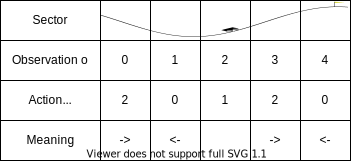
\includegraphics[width=\linewidth]{MountainCarWinner.png}
    \caption{Visual summary of the strategy enacted by \texttt{-..} on \textbf{Mountain Car}}
    \label{fig:mountaincarwinner}
\end{figure}

When the virtual comma is executed, car position and car velocity are read into memory, discretized into integers $0\dots4$.
The position is read into the active memory cell $p_T$, while the velocity is in cell $p_T+1$.
Then the active cell is decremented and the resulting number is put onto the action stack twice.
There is 1 read operation and 2 write operations to the end of the action stack, which introduces a delay before the actions get executed.
When it's time to act, the number on the action stack is coerced to one of the actions possible in this environment (0 for going left, 1 for doing nothing, 2 for right). 

A strategy emerges, illustrated on figure \ref{fig:mountaincarwinner}, in which the car puts "going right" onto the agenda if it's on the far left or the center right of the landscape, puts "going left" onto the agenda when it's on the far right or center left and schedules doing nothing if it's in the center.
This strategy helps the car successfully reach the right fringe every time it is applied.

\newpage
\section{Conclusions}

In this chapter, we have introduced a new programming language tailored to the task of programmatically interpretable reinforcement learning.
We have shown experimentally that this language can facilitate program synthesis as well as knowledge transfer between expert-based systems and data-driven systems. 

The results in the OpenAI gym test examples show that the proposed system is able to find a functional solution to the problem. In some cases the performance is similar to the best deep learning solution but the obtained program remains still explainable. This is a very encouraging result and suggest that the use of program induction methods may indeed be a viable way towards explainable solutions in RL applications. 

We propose the following directions for future work:
\begin{enumerate}
    \item Develop translation mechanisms between \textbf{BF++} and other languages. Potentially, \textbf{BF++} can be used as \emph{bytecode} \cite{bytecode} for reinforcement learning. The expert would write a program in a higher-level language and transpile it into \textbf{BF++} so that the program then can be improved with reinforcement learning.
    \item Use other neural network architectures as well as non-neural evolution methods like genetic programming \cite{genprog1,genprog2} in conjunction with \textbf{BF++}
    \item Apply the framework to problems in Healthcare where expert inspiration is important for crossing the AI chasm \cite{aichasm}.    \item Use Natural Language Generation techniques to translate the BF++ code automatically to a friendly human-readable text description as in \cite{richardsonCode2TextChallengeText2017,code2nlg2}.
\end{enumerate}

\newpage
\chapter{A Neurogenetic Programming Framework}\label{ch:neurogen}
\epigraph{I got power, poison, pain, and joy inside my DNA \\ I got hustle, though, ambition flow inside my DNA}{Kendrick Lamar}

\citeself{chapter}{liventsev2021neurogenetic}

\section{Introduction}\label{sec:neurogen-intro}


In \emph{genetic programming} \cite{genprog1,genprog2} new programs are generated by mutating and mixing a \emph{population} of programs. 
 A more recent approach, largely drawing on the earlier success of deep neural language models (see CodeBERT \cite{codebert} inspired by BERT \cite{devlinBERTPretrainingDeep2019}), have been to train black box \emph{neural models} that generate executable programs as text \cite{abolafiaNeuralProgramSynthesis2018,deepcoder,structural}. 
 Neural program synthesis and genetic programming both have unique advantages \cite{geneticvsneural}. 
 In this chapter we propose a novel hybrid of the two families of methods. We call the method \emph{Instant Scrum} in reference to a popular Agile software team work model \cite{scrum}. We show that \emph{Instant Scrum}, IS, can solve several reinforcement-guided program synthesis tasks in standard OpenAI gym benchmarks tasks (section \ref{sec:tasks}). 

After the introduction to the relevant background in the next section, we will give a detailed description of the proposed IS methodology. Next, we describe the experimental setup and the OpenAI gym test tasks, and the results of the experiments in several variations of the core IS method. Finally, we discuss the results and propose future research directions and potential applications for hybrid neurogenetic programming. 

\newpage \subsection{Programmatically Interpretable Reinforcement Learning}
\label{sec:pirl}

More concretely, we model the task as {\em Episodic Partially Observable Markov Decision Process}:

\begin{multline}
M = (\mathcal{S}_{nt}, \mathcal{S}_t, \mathcal{A}, \mathcal{O}, p_o(o | s, a), p_s(s_\text{next} | s_\text{prev}), p_r(r | s, a), p_\text{init}(s))
\end{multline}

Here, $\mathcal{S}_{nt}$ is the set of {\em non-terminal (environment) states} and $\mathcal{S}_{t}$ is the set of {\em terminal states}. 
$\mathcal{A}$ is the set of {\em actions} that the learning agent can perform, and $\mathcal{O}$ is the set of {\em observations} about the current state that the agent can make. 

A \emph{reinforcement learning episode} starts in a state $s \in \mathcal{S}_{nt}$ sampled from $p_\text{init}$, the {\em initial distribution} over environment states.
An agent action $a \in \mathcal{A}$ at the state $s$ causes the environment state to change probabilistically, and the destination state follows the distribution $p_s(\cdot | s, a)$. 
At state $s$, the probability of making observation $o$ is $p_o(o | s)$ and the probability of obtaining \emph{reward} $r$ is $p_r(r|s,a)$. 
The process continues until a $p_s$ yields a terminal state $s \in \mathcal{S}_t$.
This distinction is what sets \emph{episodic} POMDP popularized by OpenAI gym \cite{openai-gym} apart from the more traditional approach \cite{kramerjdavidrPartiallyObservableMarkov1964, spaanPartiallyObservableMarkov2012} where the process is infinite.

A \emph{program} is a sequence of tokens

\begin{equation}
    c=(c^{(1)},c^{(2)},\dots)
\end{equation}

that defines behavior of an agent.
Depending on the programming language and implementation choices the tokens can be characters or higher-level tokens, i.e. keywords.
We denote the language's \emph{alphabet}, i.e. the set of all possible tokens as $\mathcal{L}$.

An \emph{interpreter} is a tuple $\langle \alpha,\mu \rangle$ where $\mu(c_k,m_k,o_k)$ is the \emph{memorization function} that defines how the agent's memory updates upon making an observation and $\alpha(c, m_k)$ is the \emph{action function} defines which action the agent at a certain memory state takes in the POMDP.
Memory is intialized at state $m_\text{init}$

The agent's goal is maximizing total reward collected in the environment, calculated as follows:

\begin{algorithm}[H]
\begin{algorithmic}[1]
\caption{Evaluating total reward for a program}
\Function{$\mathit{Eval}$}{$c$}
\State $R_\text{tot} \gets 0$
\State $m \gets m_\text{init}$
\State $s \sim p_\text{init}(s)$
\While{$s \in \mathcal{S}_{nt}$}
\State $o \sim p_o(o | s)$
\Comment{Observe}
\State $m \gets \mu(c,m,o)$
\State $a \gets \alpha(c, m)$ 
\Comment{Act}
\State $r \sim p_r(s,a)$
\State $R_\text{tot} \gets R_\text{tot} + r$
\Comment{Get rewarded}
\State $s_\text{next} \sim p_s(s_\text{next} | s, a)$
\Comment{Next state}
\State $s\gets s_\text{next}$
\EndWhile
\State \Return $R_\text{tot}$
\EndFunction
\end{algorithmic}
\end{algorithm}

Since the algorithm for computing this function involves repeatedly sampling values from distributions, function $\mathit{Eval}(c)$ is a mapping from the set of programs to the set of real-valued random variables.

\emph{Programmatically Interpretable Reinforcement Learning} \cite{pirl} is the task of maximizing expected total reward with respect to $c$, i.e. finding a program $c$ that is best for a given POMDP environment:

\begin{equation}
    \mathbb{E}(\mathit{Eval}(c)) \longrightarrow \max_{c}
    \label{eq:pirlgoal}
\end{equation}

\newpage
\section{Methodology}

How does one manage a composition of code generators in such a way that the composition yields better programs than individual contributors are capable of? 
This question is studied extensively in software project management literature \cite{mythicalmanmonth}.
And while, admittedly, project management literature is concerned with human developers and, admittedly, there exist considerable differences between human developers and mathematical models of code generation \cite{bugfixing}, we mitigate these differences with several simplifying assumptions.

\subsection{Modeling the codebase}

Following from traditional genetic programming, we define a \emph{population} of programs. 
The \emph{codebase} is a tuple of 2-tuples, representing a program $C_c^{(i)}=c$ and the total reward it collected $C_R^{(i)}=R_\text{tot} \sim \mathit{Eval}(c)$ (see section \ref{sec:quality}):

\begin{equation}
    \mathcal{C} = \langle \langle C_c^{(1)}, C_R^{(1)} \rangle, \langle C_c^{(2)}, C_R^{(2)} \rangle \dots \langle C_c^{(|C|)}, C_R^{(|C|)} \rangle \rangle
\end{equation}

However, unlike in traditional genetic programming, the \emph{initial population} can (optionally) be empty.

\newpage \subsection{Modeling a software developer}
\label{sec:developer}

A software developer can:
\begin{enumerate}
    \item Check out programs from the codebase $\mathcal{C}$
    \item Output new a program $c$
    \item Receive feedback on their program's quality $q$ 
    \item Learn from the feedback by mofidying its strategy
\end{enumerate}

Thus, a developer is a 2-tuple of a program distribution $p_\text{dev}(c | \theta, \mathcal{C})$ and a parameter update procedure $\mathit{Update}(\theta, c, q)$

Distribution $p_{\text{dev}}(c | \theta, \mathcal{C})$ is defined over programs and is parametrized with learnable parameters $\theta$ as well as codebase $\mathcal{C}$. 
Having codebase as parameter enables the developer to generate new programs as a modification and/or combination of existing programs, i.e. to apply genetic programming.

Learnable parameters $\theta$ encode the developer's current methodology of programming that can be modified upon receipt of positive or negative feedback using the developer's update procedure. 

The \emph{team} of developers is a tuple of 2-tuples:
\begin{equation}
    \mathcal{T} = \langle \langle \mathcal{T}_p^{(1)}, \mathcal{T}_\text{upd}^{(1)} \rangle, \langle \mathcal{T}_p^{(2)}, \mathcal{T}_\text{upd}^{(2)} \rangle \dots \langle \mathcal{T}_p^{(|\mathcal{T}|)}, \mathcal{T}_\text{upd}^{(|\mathcal{T}|)} \rangle \rangle
\end{equation}

\newpage \subsection{Modeling program quality}
\label{sec:quality}

We define two empirical metrics of overall program fitness.
The first is \emph{empirical total reward}:

\begin{equation}
    R(c|\mathcal{C}) = \frac{\sum\limits_{i=1}^{|C|} \mathbb{I}[C_c^{(i)}=c] C_R^{(i)}}{\sum\limits_{i=1}^{|C|} \mathbb{I}[C_c^{(i)}=c]}
\end{equation}

If a program has been tested in the environment ($\textit{Eval()}$ function) several times, there will be several copies of it in the codebase with different quality samples.
Averaging over them yields an unbiased estimate of the expectation from equation \ref{eq:pirlgoal}, $\mathbb{E}(\mathit{Eval}(c))$, that we set out to maximize.

The second is \emph{empirical program quality}, defined as

\begin{equation}
    Q(c|\mathcal{C}) = \frac{\sum\limits_{i=1}^{|C|} \mathbb{I}[C_c^{(i)}=c] e^{C_R^{(i)}}}{\sum\limits_{i=1}^{|C|} \mathbb{I}[C_c^{(i)}=c]}
    \label{eq:empquality}
\end{equation}

\emph{Empirical program quality} is an unbiased estimate of $\mathbb{E}(e^{\mathit{Eval}(c)})$
The idea behind exponentiating the total reward is to encourage \emph{exploration} \cite{exploration}.
Programs that on average perform poorly, but sometimes, stochastically, collect high rewards, will have a higher $Q(c|C)$ than $R(c|C)$.
We consider these programs to be \emph{high-quality additions to the codebase} because they contain the knowledge necessary for solving environment $M$, even if on average they don't solve it.
We hypothesize that applying \emph{genetic operators} (section \ref{sec:genetic}) to programs with high $Q(c|C)$ can yield programs with high $R(c|C)$.
For this reason we train developers to maximize $Q$, but when the training is complete, we pick programs from the codebase with the highest $R$ as "best programs".
 
$Q(c|C)$ has an additional technical advantage over $R(c|C)$: invariant $Q(c|C) \geq 0$ holds for all $c$.
This lets one sample programs from the codebase with probabilities proportional to their quality, see eq. \ref{eq:genmixture}.

\newpage \subsection{Populating the codebase}

Just like \emph{instant run-off voting} achieves similar results to \emph{exhaustive ballot runoff voting}, but does it much faster by replacing a series of ballots cast in a series of elections with a ballot cast once that goes on to participate in a series of virtual elections \cite{votingsystems}, our \emph{Instant Scrum} algorithm does the same to Scrum \cite{scrum}: it simulates the iterative software development process recommended by Scrum methodology without humans in the loop making it possible to run many sprints per second:

\begin{algorithm}[H]
\begin{algorithmic}[1]
\caption{Instant Scrum with a team of developers}
\label{alg:instantscrum}
\Procedure{InstantScrum}{$T,\mathcal{C},N_\text{max}$}
\State $N \gets 0$
\While{$N < N_\text{max}$}
\LineComment{For each developer in the team}
\For{$i = 1,2,\dots,|T|$}
\LineComment{Sample a program from the developer}
\State $c_\text{new}\sim p_i(c | \theta_i, \mathcal{C})$ 
\LineComment{Test the program}
\State $R_\text{tot} \gets \mathit{Eval}(c_\text{new})$
\LineComment{Save the code and test result to the codebase}
\State $\mathcal{C} \gets \mathcal{C} \cup \{\langle c_\text{new}, R_\text{tot} \rangle\}$
\LineComment{Train the developer}
\State $\mathit{Update}_i(\theta_i, c, q)$
\LineComment{Increment sprint counter}
\State $N \gets N+1$
\EndFor
\EndWhile
\EndProcedure
\end{algorithmic}
\end{algorithm}

To combine genetic programming and neural program synthesis we introduce 3 types of developers: \emph{genetic} and \emph{neural} and \emph{dummy}, create a team that contains developers of all types and run \emph{Instant Scrum}.

\newpage \subsection{Genetic developers}
\label{sec:genetic}

A genetic developer writes programs by
\begin{enumerate}
    \item Selecting one of the 7 available stochastic \emph{genetic operators} (described below)
    \item Selecting two programs from the \emph{codebase} $C$ (parents $c_1$ and $c_2$) 
    \item Using the operator to modify the parents and yield a new (child) program
\end{enumerate}

A genetic operator is a probability distribution $p_\text{op}$ over child programs given 2 parent programs. 

\begin{equation}
    p_\text{op}(c_\text{child}|c_1,c_2)
\end{equation}

Operators whose $p_\text{op}$ is invariant to $c_2$ and depends on $c_1$ only are called \emph{mutation} operators: they generate a new program by \emph{mutating} one program $c_1$.
The rest are called \emph{combination} operators as they \emph{combine} 2 existing programs to generate a new one.



\paragraph{Mutation operators}

The simplest method for randomly modifying a program is \emph{shuffle mutation}: randomly re-order the tokens of $c_1$.
Let $\mathrm{A}$ be the set of all possible permutations of size $|c_1|$. $|\mathrm{A}|=|c_1|!$. 
Then

\begin{equation}
    p_\text{shuffle}(c_\text{child}|c_1,c_2) =
            \frac{\sum\limits_{\alpha \in \mathrm{A}} \mathbb{I}[\alpha(c_\text{parent}) = c_\text{child}]}{|c_1|!}
\end{equation}

Another approach is \emph{uniform mutation} where a loaded coin is tossed for every token in $c_1$. 
With probability $p_\text{ind}$ it is replaced with a random token from the alphabet $\mathcal{L}$ of the programming language, with probability $1-p_\text{ind}$ it stays the same.
The evolution of a single token under shuffle mutation is defined by distribution

\begin{equation}
    p(c^\text{new} | c^\text{old}) = \frac{p_\text{ind}}{|L|} +  (1 - p_\text{ind}) \mathbb{I}[c^\text{new} = c^\text{old}]
\end{equation}

Hence over full programs the operator is defined as

\begin{equation}
    p_\text{unimut}(c_\text{child}|c_1,c_2) = \mathbb{I}[|c_\text{child}|=|c_1|] \\ 
    \prod\limits_{i=0}^{|c_1|}  \left(\frac{p_\text{ind}}{|L|} +  (1 - p_\text{ind}) \mathbb{I}[c_\text{child}^{(i)} = c_1^{(i)}] \right)
\end{equation}

\paragraph{Combination operators}

The combination operators we propose are all variants of \emph{crossover} - a classic genetic programming technique rooted in the way a pair of DNA molecules exchanges genes during mitosis and meiosis, displayed on figure \ref{fig:crossover}.

In DNA \cite{evocritique}, as well as in most genetic programming literature \cite{genprog1,genprog2} the crossover operator combines 2 parent sequences to produce 2 children.
In this section, in order to reduce complexity, we define the distributions as if only the first child program is saved and the second one is forgotten.
Since program pair $\langle c_2, c_1 \rangle$ is equally likely to be selected for combination as $\langle c_1, c_2 \rangle$ (see eq. \ref{eq:genmixture}) this modification does not affect the resulting genetic developer distribution.

In \emph{one-point crossover} a random cut position $k$ is selected and the trailing sections of 2 parent programs beginning with the cut point are swapped with each other. 
If the parent programs have different lengths, the cut point has to fit within both programs:

\begin{equation}
    2 \leq k \leq |c_1,c_2|; |c_1,c_2| = \min\{|c_1|, |c_2|\}
\end{equation}

Hence the probability of $c_\text{child}$ being born out of \emph{one-point crossover} is

\begin{equation}
    p_\text{1ptcx}(c_\text{child}|c_1,c_2) =
        \frac{\mathbb{I}[|c_\text{child}|=|c_2|]}{|c_1,c_2|-1}
        \sum\limits_{k=2}^{|c_1,c_2|} \prod\limits_{i=1}^{k-1} \mathbb{I}[c_\text{child}^{(i)} = c_1^{(i)}] \prod\limits_{i=k}^{|c_2|} \mathbb{I}[c_\text{child}^{(i)} = c_2^{(i)}]
\end{equation}

\emph{Two-point crossover} is similar, but instead of swapping the trailing ends of programs, a section in the middle of the programs is chosen, determined by randomly selected cut-off indices $k_1$ and $k_2$ and swapped:

\begin{equation}
\begin{split}
    p_\text{2ptcx}(c_\text{child}|c_1,c_2) = // =
        \frac{2 \mathbb{I}[|c_\text{child}|=|c_1|]}{(|c_1,c_2|-2)(|c_1,c_2|-1)}
        \sum\limits_{k_1=2}^{|c_1,c_2|-1}
        \sum\limits_{k_2=k_1+1}^{|c_1,c_2|} \\
        \prod\limits_{i=1}^{k_1-1} \mathbb{I}[c_\text{child}^{(i)} = c_1^{(i)}] \prod\limits_{i=k_1}^{k_2-1} \mathbb{I}[c_\text{child}^{(i)} = c_2^{(i)}]
        \prod\limits_{i=k_2}^{|c_1|} \mathbb{I}[c_\text{child}^{(i)} = c_1^{(i)}]
\end{split}
\end{equation}

\emph{Uniform crossover} mirrors \emph{uniform mutation} in that a loaded coin is tossed for each token in $c_1$. With probability $p_\text{ind}$ the token is replaced, but the replacement is not drawn randomly from the alphabet. Instead, the replacement comes from $c_2$:

\begin{equation}
    p_\text{unicx}(c_\text{child}|c_1,c_2) = \prod\limits_{i=0}^{|c_1|} \mathbb{I}[|c_\text{child}|=|c_1|] \\ \left(p_\text{ind} \mathbb{I}[c_\text{child}^{(i)} = c_2^{(i)}] + (1 - p_\text{ind}) \mathbb{I}[c_\text{child}^{(i)} = c_1^{(i)}] \right)
\end{equation}

Finally, \emph{messy crossover} is a version of \emph{one-point crossover} without the assumption that both parent programs have to be cut at the same index $k$.
In \emph{messy crossover}, one parent is cut at index $k_1$, another is cut at index $k_2$ and the head of one is attached to the tail of the other:

\begin{multline}
    p_\text{messy}(c_\text{child}|c_1,c_2) =
        \frac{1}{(|c_1,c_2|-1)^2}
        \sum\limits_{k_1=2}^{|c_1,c_2|} \sum\limits_{k_2=2}^{|c_1,c_2|} \\ \mathbb{I}[|c_\text{child}|=k_1+|c_2|-k_2] \\ \prod\limits_{i=1}^{k_1-1} \mathbb{I}[c_\text{child}^{(i)} = c_1^{(i)}] \prod\limits_{i=1}^{|c_2|-k_2} \mathbb{I}[c_\text{child}^{(k_1+i)} = c_2^{(k_2+i)}]
\end{multline}

\begin{figure}
    \centering
    \includegraphics[width=0.45\linewidth]{Morgan_crossover_1.jpg}
    \includegraphics[width=0.5\linewidth]{Morgan_crossover_2.jpg}
    \caption{1-point and 2-point crossover \cite{evocritique}}
    \label{fig:crossover}
\end{figure}

\begin{table}
    \centering
    \begin{tabular}{r|l}
         Parent 1 & \color{blue}\verb|ae>>>>>34+| \\
         Parent 2 & \color{red}\verb|a[e>-a-]b[e>>-b-]| \\
         \midrule
         Shuffle mutation & \color{blue}\verb|>>4+>3>e>a| \\
         Uniform mutation & \color{blue}\verb|ae|\color{black}\verb|@|\color{blue}\verb|>|\color{black}\verb|!|\color{blue}\verb|>>3|\color{black}\verb|5|\color{blue}\verb|+| \\
         1-point crossover & \color{blue}\verb|ae>>>>|\color{red}\verb|-]b[e>>-b-]| \\
         2-point crossover & \color{blue}\verb|ae>|\color{red}\verb|>-a-|\color{blue}\verb|34+| \\
         Uniform crossover & \color{blue}\verb|ae|\color{red}\verb|e|\color{blue}\verb|>|\color{red}\verb|-|\color{blue}\verb|>>3|\color{red}\verb|b|\color{blue}\verb|+| \\
         Messy crossover & \color{blue}\verb|ae>>>>|\color{red}\verb|e>-a-]b[e>>-b-]| \\
         Pruning & \color{blue}\verb|e>>>>>4+| \\
    \end{tabular}
    \caption{All operators applied a pair of BF++ programs}
\end{table}


\paragraph{Pruning operator}

After initial experiments  we found that generated programs often contain sections of unreachable code or code that makes changes to the execution state and fully reverses them.
To address this, we introduced an additional operator for removing dead code (\emph{pruning}): when Instant Scrum encounters a successful program, pruning helps separate sections of this program that led to its success from sections that appeared in a highly-rated program by accident.  

Implementation of the pruning operator depends on the programming language at hand, here we define it as a pruning function $c_\text{pruned}=\mathit{Prune}(c_1)$ that outputs a program functionally equivalent to $c_1$ (memory functions $(\alpha,\mu)$ of $c_\text{pruned}$ are equal to that of $c_1$) and $|c_\text{pruned}| \leq c_1$ and a degenerate probability distribution:

\begin{equation}
    p_\text{prune}(c_\text{child}|c_1,c_2)= \begin{cases}
        1 & c_\text{child} = \mathit{Prune}(c_1) \\
        0 & \text{otherwise}
        \end{cases}
\end{equation}

\paragraph{Operator and parent selection}
\label{sec:selection}

Let $\mathcal{P}_\text{genetic}$ be a tuple of all available genetic operators, in order of introduction, i.e. $\mathcal{P}_\text{genetic}^{(1)}=p_\text{shuffle}$ and $\mathcal{P}_\text{genetic}^{(4)}=p_\text{2ptcx}$

Genetic developer's program distribution is a mixture distribution, combining different operators that can be applied, weighted by learnable parameters, and different programs that can be sampled from the codebase, weighted by \emph{empirical quality} (eq. \ref{eq:empquality}).

\begin{equation}
    p_\text{genetic}(c | \theta, \mathcal{C}) = 
    \sum\limits_{c_1}^{C}  
    \sum\limits_{c_2}^{C} 
    \frac{Q(c_1|C) Q(c_2|C)}{(\sum\limits_{c}^{C} Q(c|C))^2} 
    \sum\limits_{i=0}^{|\mathcal{P}_\text{genetic}|} 
    \theta_i \mathcal{P}_\text{genetic}^{(i)} (c|c_1,c_2)
    \label{eq:genmixture}
\end{equation}

This is a true probability distribution if and only if $\sum\limits_{i=0}^{|\mathcal{P}_\text{genetic}|} 
    \theta_i = 1$


\paragraph{Training the genetic developer}

One challenge that remains to be solved to fully define the genetic developer (folowing section \ref{sec:developer}) is to define a learning from feedback strategy $\mathit{Update}_\text{genetic}$.
To do this, we notice that equation \ref{eq:genmixture} contains a \emph{multi-armed bandit} \cite{banditproblem} hiding in plain sight.
Indeed, once the \emph{genetic} developer samples $c_1$ and $c_2$ from the codebase, it has to pick one of 7 available options (pull one of 7 \emph{levers}) to then receive a reward $\mathit{Eval}(c_\text{child})$.
This subproblem can be represented with a POMDP of its own and solved using one of the standard bandit algorithms \cite{banditsolutions}.

Following \emph{Occam's razor}, we picked the simplest method, \emph{epsilon-greedy optimization}: we calculate the value of each operator as mean total reward of programs generated with this operator:

\begin{equation}
    V^{(i)} = \frac{1}{|\mathcal{C}(\mathcal{P}_\text{genetic}^{(i)})|} 
    \sum\limits_{k=1}^{|\mathcal{C}(\mathcal{P}_\text{genetic}^{(i)})|}
    \mathcal{C}(\mathcal{P}_\text{genetic}^{(i)})_R^{(k)} 
\end{equation}

where $C(\mathcal{P}_\text{genetic}^{(i)})$ is the subset of the codebase produced via operator $\mathcal{P}_\text{genetic}^{(i)}$.

The $\mathit{Update}_\text{genetic}$ procedure recalculates values $V$ and sets operator probabilities to

\begin{equation}
    \theta_i = \frac{\epsilon}{|\mathcal{P}_\text{genetic}^{(i)}|} +
    \mathbb{I}[i = \underset{i}{\arg\max} V^{(i)}] (1 - \epsilon)
\end{equation}

where $\epsilon$ is a hyperparameter responsible for regulating the \emph{exploration-exploitation tradeoff} \cite{banditsexplo}

In future work, however, other bandit optimization algorithms can be used in its place \footnote{Our open-source software implementation allows for drop-in replacement of bandit algorithms}.

\paragraph{Hyperparameters}
\label{sec:genhyper}

The genetic developer, as described above, has 2 hyperparameters:

\begin{enumerate}
    \item $p_\text{ind}$ defines severity of mutation in $p_\text{unimut}$ and $p_\text{unicx}$
    \item $\epsilon$ defines learnability of genetic operator distribution
\end{enumerate}

Note that the \emph{team} mechanism afforded by \emph{Instant Scrum} can be used not only to combine genetic and neural program synthesis, but also to combine several genetic developers with different hyperparameters.

\newpage \subsection{Neural developers}
\label{sec:neural}

The \emph{neural developer}, also known as the \emph{senior developer} because of their unique ability to write original programs, is an LSTM \cite{hochreiterLongShorttermMemory1997} network followed by a linear layer that generates a sequence of vectors $h_{1},h_{2},h_{3},\dots$ where $h_i \in \mathbb{R}^{|\mathcal{L}| + 1} \forall i$ and $j$-th element of vector $h_i$, $h_i^{(j)}$, represents the probability of $i$-th token of the program being $j$-th token in the alphabet, $p(c^{(i)}=\mathcal{L}^{(j)})$.
The last element of the vector represents a special \emph{end of program} symbol.
This vector depends deterministically on the full set of neural network parameters (LSTM and linear layer) $\theta$ and can be represented as a function $h_i(\theta)$.
Then

\begin{equation}
    p_\text{neural}(c | \theta, \mathcal{C}) = h_{(|c|+1)}^{\mathcal{L}+1}
    \prod\limits_{i=1}^{|c|}
    \sum\limits_{j=1}^{|\mathcal{L}|} \mathbb{I}[c^{(i)}=\mathcal{L}^{(j)}]
    h_i(\theta)
\end{equation}

For the $\mathit{Update}_\text{neural}$ procedure we use the algorithm proposed in \cite{abolafiaNeuralProgramSynthesis2018}.
The subproblem of generating a program $c$ is considered as a reinforcement learning episode of it's own, where tokens are actions and token number $|c|+1$ (\emph{end of program} token) is assigned reward $q = e^R; R \sim Eval(c)$. 
In this subenvironment $h_i(\theta)$ is the policy network \cite[chapter 13]{suttonReinforcementLearningSecond2018} trained using REINFORCE algorithm with Priority Queue Training.
This algorithm involves a priority queue of best known programs: we implement it as programs from $C$ with highest $Q(c|C)$ which means that the neural developer can train on programs written by other developers.

$h_i(\theta)$ can also represent several LSTM layers stacked or a different type of recurrent neural network, i.e. GRU \cite{choPropertiesNeuralMachine2014,chung2014empirical}.
Hyperparameters of this neural network, such as hidden state size and/or number of stacked layers are hyperparameters of the neural developer.  

\newpage \subsection{Dummy developer}

The last developer we introduce is the simplest one:

\begin{equation}
    p_\text{dummy}(c_\text{child}|c_1,c_2) = 
    \frac{Q(c_\text{child}|C)}{\sum\limits_{c}^{C} Q(c|C)} 
    \label{eq:dummy}
\end{equation}

Dummy developer does not generate novel programs.
Instead, it uses the same quality-weighted program sampling as in equation \ref{eq:genmixture} to decide which existing program to copy.
Their utility may not be obvious at first, but note (section \ref{sec:quality}) that when the same program is added to the codebase several times, it's total reward and quality estimates are averaged and grow more accurate.

Dummy developer is a smart compromise between speed at which \emph{Instant Scrum} (algorithm \ref{alg:instantscrum}) is searching the program space and the quality of its working map of the program space, focusing on its most "interesting" (high $Q(c|C)$) parts. 
Without dummy developer, all empirical total rewards $E[Eval(c)]$ would be low quality estimates of true fitness of the program and one spurious success of an otherwise bad program could steer the search in the wrong direction.
On the other hand, we could test each program many times before adding it to the codebase, but that would slow down the search prohibitively. 

\newpage
\section{Experimental setup}
\label{sec:neurogen-experiments}

\paragraph{Teams}

In the table below, we introduce 5 teams.
Neural developers are denoted as lstm(hidden state dimensionality), several numbers mean a stacked LSTM.
Genetic developers are denoted as $\text{gen}(p_\text{ind},\epsilon)$, see secion \ref{sec:genhyper}.
$T_\text{small}$ and $T_\text{large}$ are recommended configurations while $T_\text{genetic}$, $T_\text{neural}$ are \emph{ablation studies} to prove that combination of neural and genetic methods is useful.

\begin{table}[H]
\centering
\begin{tabular}{r|c|c|c|c}
     Developer & $T_\text{small}$ & $T_\text{large}$ & $T_\text{genetic}$ & $T_\text{neural}$  \\
     $\text{lstm}(10)$ & & \checkmark & & \\
     $\text{lstm}(50)$ & & \checkmark & & \\
     $\text{lstm}(256)$ & & \checkmark & & \\
     $\text{lstm}(10,10)$ & & \checkmark & & \\
     $\text{lstm}(50,50)$ & \checkmark & \checkmark & & \checkmark \\
     $\text{lstm}(256,256)$ & & \checkmark & & \\
     $\text{gen}(0.2,0.2)$ & \checkmark & &  & \\
     $\text{gen}(\frac{1}{3},0.2)$ & & \checkmark & & \\
     $\text{gen}(\frac{1}{6},0.2)$ & & \checkmark & & \\
     $\text{gen}(\frac{1}{12},0.2)$ & & \checkmark & & \\
     dummy & \checkmark & \checkmark & \checkmark & \checkmark \\
\end{tabular}
\caption{Team composition}
\end{table}


\paragraph{Language}

Instant Scrum can be used to generate programs in any programming language provided:
\begin{enumerate}
    \item An interpreter $\langle \alpha,\mu \rangle$, see section \ref{sec:pirl}
    \item A known finite alphabet $\mathcal{L}$
    \item A pruning function $\mathit{Prune}(c)$
\end{enumerate}

%Moreover, pruning function and finite alphabet are, in a sense, optional requirements: pruning isn't essential to the method, so a dummy pruning function $P(c)=c$ can be used instead and if a language's alphabet is infinite, it is usually possible to develop a reasonable finite subset of the full alphabet and generate programs in it.

% Ode to BF++

% A word on trees
The complexity of the chosen language is important since in complex languages random perturbations of program source code often produce grammatically invalid programs.
This issue has been addressed with \emph{structural models} \cite{grammargp,structural} \cite[chapter 4]{genprog1}, however, we sidestep the issue entirely by using \emph{BF++} (see chapter \ref{ch:bfpp}) - a simple language developed for \emph{programmatically interpretable reinforcement learning} where most random combinations of characters are valid programs.
Each BF++ command is represented with a single character, thus the only way to tokenize it is to let tokens $c^{(1)},c^{(2)},c^{(3)},\dots$ be single characters.

\paragraph{Tasks}
\label{sec:tasks}

Following from the previous chapter we synthesize programs for \textbf{CartPole-v1} \cite{cartpole}, MountainCarContinuous-v0 (\textbf{MCC-v0}) \cite{mountain_car}, \textbf{Taxi-v3} \cite{taxi} BipedalWalker-v2 (\textbf{BW-v2})  OpenAI Gym \cite{openai-gym} environments, see figure \ref{fig:envs}.

\paragraph{Initial populations}

Where possible, we run all experiments twice - a control experiment with empty intial codebase, and an experiment where codebase is pre-populated with human-written programs from chapter \ref{ch:bfpp}.
Exceptions to this rule are 
\begin{itemize}
    \item Teams $T_\text{genetic}$ and $T_\text{pure}$ that only have code modification (not generation) capability and thus require initialization 
    \item \textbf{BipedalWalker-v2} environment, because this environment proved challenging to manually develop BF++ for (see chapter \ref{ch:bfpp})
\end{itemize}

\paragraph{Stopping and scoring}

For Taxi we set an $N_\text{max}$ to $100000 |T|$ sprints, meaning every developer in the team trains for 100000 iterations.
For other tasks we used Exponential Variance Elimination \cite{evestop} early stopping algorithm to stop the process when the positive trend in $Eval(c)$ is not present for 10000 sprints.
This approach rules out the hypothesis that \emph{Instant Scrum} is equivalent to enumerative search and it finds good programs by exhaustion as opposed to learning - if that was the case, early stopping would fire immediately.
Taxi environment is treated differently because programs that cannot pick up and drop off at least one passenger are always rewarded with -200 and at first it takes many iterations to synthesize at least one program that can.
In addition to these stopping rules, a hard timelimit was set.

After the process is stopped, we pick 100 programs with the highest $R(c|C)$ and make sure each of them has been tested at least 100 times, otherwise we run $Eval(c)$ and add result to the codebase until 100 samples is reached. 

\paragraph{Implementation}

We implemented the framework with Python and Tensorflow as well as DEAP \cite{deap} for genetic operators.

\newpage
\section{Results}
\label{sec:neurgen-results}

\begin{table*}[]
    \centering
    \begin{tabular}{c|c|c|c|c|c|c|c}
         Environment & \multicolumn{2}{c}{CartPole-v1} & \multicolumn{2}{c}{MCC-v0} & \multicolumn{2}{c}{Taxi-v3} & BW-v2 \\
         Initial programs & & 20.48 & & -6.55 & & -150.44 & \\
         \midrule
         $T_\text{small}$  &    60.93 &    143.91 &     \textbf{92.53} &     88.20 &   -148.23 &   -150.44 &     -0.16\\
         $T_\text{large}$ & \textbf{157.35} &     57.47 &     91.65 &     91.42 &    \textbf{-32.12} &   -150.44 &      \textbf{8.13} \\ 
         $T_\text{genetic}$& - & 59.12 & - & 0 & - & -47.54 & - \\ 
         $T_\text{neural}$ & 71.38 & 96.64 & 88.41 & 91.38 & -198.9 & -150.44 & 6.17 \\
         \midrule
         Leaderboard threshold & 195 & 195 & 90 & 90 & 0 & 0 & 300 \\ 
    \end{tabular}
    \caption{Averaged 100-episode reward acheived by the best program in each category}
    \label{tab:results}
\end{table*}

See table \ref{tab:results} for a summary of best programs generated.
The metric used, average $R$ over 100 evaluations is the same metric that's used in the OpenAI gym leaderboard, so we include the threshold required to join the leaderboard for context.
\emph{Initial programs} refers to the best program in the codebase before \emph{Instant Scrum} starts when it is prepopulated with  programs from chapter \ref{ch:bfpp}.

The main hypothesis of this chapter is \textbf{confirmed}: neurogenetic approach is superior to neural program induction or genetic programming separately.

Besides, one unintuitive result of our experiments is that initialization of the codebase with previously available programs can be harmful, see $T_\text{large}$.
Overall, best results were acheived without inspiration from human experts, however, it is very valuable for lightweight teams with few small (in terms of $|\theta|$) developers.

Additionally, we can examine in more detail how single developers compare to each other (and notice that only neural developers are on the list): 

\begin{table}[H]
\centering
\begin{tabular}{r|c|c|l}
    Task & Init & $R(c|C)$ & Developer \\
    \midrule
    CartPole-v1 & & 157.35 & lstm(256) \\
CartPole-v1 & \checkmark & 57.47 & lstm(256,256) \\
MountainCar & & 91.65 & lstm(10,10) and pruning \\
MountainCar & \checkmark & 91.42 & lstm(50) \\
Taxi-v3 & & -32.12 & lstm(50) \\
Taxi-v3 & \checkmark &  -150.44  & human \\
BipedalWalker-v2 & & 8.13 & lstm(256,256) \\
\end{tabular}
\caption{Members of $T_\text{large}$ that generated the best program}
\end{table}

The same is true for $T_\text{small}$:

\begin{table}[H]
\centering
\begin{tabular}{r|c|c|l}
    Task & Init & $R(c|C)$ & Developer \\
    \midrule
    CartPole-v1 & & 60.93 & lstm(50,50)  \\
CartPole-v1 & \checkmark & 143.9 & lstm(50,50) \\
MountainCar & & 92.53 & lstm(50,50) \\
MountainCar & \checkmark & 88.2 & lstm(50,50) \\
Taxi-v3 & & -148.23 & $\text{gen}(0.2,0.2)$, $p_\text{unicx}$ \\
Taxi-v3 & \checkmark & -150.44 & human \\
BipedalWalker-v2 & & -0.15 & lstm(50,50)\\
\end{tabular}
\caption{Members of $T_\text{small}$ that generated the best program}
\end{table}

However, comparing results for $T_\text{small}$ versus $T_\text{neural}$ proves that genetic developers have been intstrumental to the quality of these neural networks - this is to be expected with Priority Queue Training (see sec. \ref{sec:neural}).

\newpage
\section{Discussion}

We have introduced a neurogenetic programming framework, demonstrated its efficacy and advantages over simpler program induction methods.

We believe that this framework can become a basis for many future methods - new methods of program synthesis can be built into the \emph{Instant Scrum} framework as developers and combined with existing ones as necessary.
In particular, one type of developer currently absent from our experiments is a \emph{neural mutation} - a neural network that modifies existing programs and can be trained to modify them in a way that improves their performance.
Another important direction is applying the framework to more specialized tasks like robotics or healthcare decision support. 

\newpage
\chapter{A Tree Variational Autoencoder for Code}\label{ch:tree2tree}
\input{sections/autocode/autoenc}

\newpage
\chapter{A Multiagent Framework for Programming with Large Language Models}\label{ch:seidr}
\input{sections/autocode/autoregr}

% =======================================================================================
%                                   PART II
% =======================================================================================
\part{For Personal Health}
%----------------------------------------------------------------------------------------
\newpage
\chapter{The Promise} \label{ch:health-motiv}
% Importance of Smart Healthcare
Understaffing has been consistently identified as the major challenge facing Healthcare today \cite{ashleyy.metcalfHospitalUnitUnderstaffing2016,SurveyShowsHidden1993,UnderstaffingSignificantIssue2012,campbell_universal_2013, hudsonUnderstaffing2015, mercerMessageEditorinChief2008, r.stanleyUnderstaffedOverwhelmed2010, munnUnderstaffingWardsCompromising2017, thelancetHealthcareSystemStaffing2018}. Automation tools that make use of Machine Learning (also known as Healthcare 4.0 \cite{tortorellaHealthcareTrendsChallenges2020}) have been consistently identified as crucial for reducing the workload of Healthcare professionals and improving the quality of care \cite{agrawalMachineLearningHealthcare2020, deviDesignImplementationAdvanced2022, g.kumarSurveyMachineLearning2016, ganguliMachineLearningPursuit2020, maityMachineLearningImproved2017, mitraMachineLearningHealthcare2021, pianykhImprovingHealthcareOperations2020, xhaferraRoleMachineLearning2022}. In turn, the shortage of standard benchmarks has been consistently identified as a central roadblock for machine learning in Healthcare \cite{Crown2015Potential, David2020Evaluating, Gu2023Beyond, Harutyunyan2019Multitask, Kathrin2022Benchmark, liventsevEffectivePatientSimulators2021, McDermott2021Reproducibility, Purushotham2018Benchmarking, S2017Benchmark}.

Whether it's ImageNet \cite{dengImagenetLargescaleHierarchical2009} in Computer Vision or GLUE \cite{wangGLUEMultitaskBenchmark2018} in natural language processing, benchmarks are a core research tool in mature applications of machine learning, enabling quantitative analysis of learning methodologies to guide and orient their development.
Machine learning for Healthcare, an emergent field with unique challenges in availability of research datasets \cite{Anshik2021Handling, Gilbert2015market, Pahwa2021Big, Yazhini2019State} lacks an accepted benchmarking standard: recent literature reviews \cite{palMachineLearningHealthcare2023,tortorellaHealthcareTrendsChallenges2020} of the field cover a variety of studies that each use their own (often non-public) benchmark.

The lack of benchmarks is a crucial barrier to advancing the quality and accessibility of care with automatic programming. 
The most promising approach for advancing Healthcare with program synthesis is
\begin{enumerate}
    \item Use clinical data, such as electronic health records, to train a patient simulator: a predictive model of patient’s future health conditional on clinicians’ decisions. 
    \item Use Programmatically Interpretable Reinforcement Learning to search for a program/protocol that performs well in that simulator.
\end{enumerate}

Having developed a sufficiently robust PIRL algorithm, let us now turn our attention to part (1) - effective patient simulators.

\newpage
\chapter{The State of the Art} \label{ch:health-sota}
Automatic program synthesis has been a long term goal of the field of artificial intelligence since its inception \cite{mannaAutomaticProgramSynthesis1971}, promising to reduce the workload of software developers by automatically solving some of the tasks they face.
And since the field's inception it has been grappling with the challenging properties of the sparse optimization space \cite{alurSyntaxguidedSynthesis2013, davidProgramSynthesisChallenges2017} that is the set of all programs in a certain programming language, namely, 
\begin{enumerate}
    \item valid error-free programs constitute an exceedingly small part of the space of possible strings, so any program synthesis algorithm that incorporates random guessing (for instance, Reinforcement Learning with random initialization \cite{suttonReinforcementLearningSecond2018}) is exceedingly unlikely to guess a valid program;
    \item a small edit in a program can result in a large difference in it's behavior (and, conversely, the same algorithm can be expressed with very different programs), hence the programs we would like to find are not clustered in any compact part of the optimization space;
    \item some of the evaluation mechanisms of programs, especially in the \emph{Programmatically Interpretable Reinforcement Learning} paradigm involve stochasticity and can yield different results for the same program.
\end{enumerate}

In other words, the search space in program synthesis is \emph{sparse}, \emph{brittle} and sometimes \emph{noisy} \cite{arnoldNoisyOptimizationEvolution2002} - all known challenges in Optimization Theory.

\newpage
\section{Genetic programming}

\begin{figure}[H]
    \centering
    \includegraphics[width=\linewidth]{gp.png}
    \caption{Genetic Programming, schematic definition}
    \label{fig:gp}
\end{figure}

The family of optimization methods best applicable to this type of complex non-differentiable search space is \emph{genetic and evolutionary methods} - biologically inspired methods that operate on a population of candidate solutions (programs), randomly edit (\emph{mutation}) and combine (\emph{recombination}) to expand the population and the prune the population by \emph{natural selection}: removing the candidates that adhere to the specification the least.
Within program synthesis this family of methods is known as \emph{genetic programming} \cite{genprog1, genprog2, genprogast}
In an evolutionary setting, as soon as at least one (preferably several) valid program is found, initializing the population to include them drastically speeds up the search process, thus addressing the sparsity issue.
This approach is particularly powerful in a setting where some solutions are already known, but a program synthesis system can be used to search for solutions that fit the \emph{specification} even better, a setting known as \emph{genetic improvement of software} \cite{petke2018:genetic}.

Genetic programming has been successfully applied in various domains, including prediction and control \cite{dracopoulosGeneticProgrammingPrediction1997}, the synthesis of complex structures (Koza, 2003), and the evolution of neural network modules \cite{degarisGENETICPROGRAMMING1990}. In the field of engineering, genetic programming has been applied to systems modeling, control, optimization, scheduling, design, and signal processing \cite{willisGeneticProgrammingIntroduction1997}. 

The biggest drawback of GP is that it requires generation and evaluation of a very high number of programs: higher than most other methods (see chapter \ref{ch:seidr}).
If evaluation of a generated program is computationally expensive, this translates directly into a very high computational cost of program synthesis.

\newpage
\section{Constrained programming languages}

Another way to address the complexity of the search space is to select a programming language such that the space of possible programs in that programming language exhibits less of the undesirable properties of optimization spaces.
For examples, a language where any combination of valid characters is a valid program \cite{brainfuck} eliminates a significant share of the complexity of the problem.
This family of approaches is explored in more detail in chapter \ref{ch:bfpp}, including  introduction of a novel constrained programming language for \emph{programmatically interpretable reinforcement learning}

\paragraph{Domain specific languages}

\cite{fowlerDomainspecificLanguages2010, hudakDomainspecificLanguages1997, karsaiDesignGuidelinesDomain2014, kosarComparingGeneralpurposeDomainspecific2010, kosarDomainspecificLanguagesSystematic2016, mernikWhenHowDevelop2005}

\paragraph{Logic programming}

One domain that's particularly amenable to solving synthesis tasks is logic programming:  a programming paradigm based on formal logic \cite{doetsLogicLogicProgramming1994, lloydFoundationsLogicProgramming2012}. 
In constrast to other programming paradigms \cite{floydParadigmsProgramming2007, gorodniaiaStudyProgrammingParadigms2016, krishnamurthi13ProgrammingParadigms2019, vanroyProgrammingParadigmsDummies2009} 

Instead of (or in addition to) generating a program first and testing whether it adheres to specification, \emph{deductive} methods apply equivalence rules to translate the specification into an executable.
This is hard to apply in \emph{programmatically interpretable reinforcement learning} where the specification is a black box, but can be a powerful approach in \emph{code translation} and \emph{programming by example} paradigms.



\newpage
\section{Pre-training methods}

\emph{Inductive synthesis}

\emph{concept space}

The paradigm of foundation models \cite{foundation-models} has recently been very prominent in machine learning and machine learning on source code is no exception.
In this paradigm, a model is first trained on a large dataset to solve a generic task such as next-token prediction and then used as a central component in solutions of various specific tasks.
The foundation models for source code, based on architectures such as GPT Codex \cite{radfordImprovingLanguageUnderstanding,chenEvaluatingLargeLanguage2021,codegen,gpt-neo} and BERT \cite{devlinBERTPretrainingDeep2019,codebert} have enabled significant process in tasks like programming by example \cite{halbertProgrammingExample1984} and even human-comparable performance in coding competitions \cite{liCompetitionLevelCodeGeneration2022}.

\paragraph{Autoregressive models}


\paragraph{Autoencoder models}

While undoubtedly useful in many program synthesis tasks, popular foundation models may fall short in the areas of genetic programming \cite{genprogast} and genetic improvement of software \cite{petke2018:genetic}.
In this settings, new programs are found by exploring the space of programs similar to one or several reference programs.
The task of applying these perturbations to programs could benefit from a foundational model, however, it's unclear how to achieve this with the current autoregressive models.
Autoencoder Genetic Programming \cite{autoenc-gp,denoising-autoenc-gp,latentspaceopt} argues for using autoencoder \cite{autoencoders} models instead.
These models embed programs into a high-dimensional vector space, making it easy to mutate a program by add random noise to the embedding vector or combine several programs by averaging their embedding vectors.

\newpage
\section{Grammar guided synthesis}

Another way to constrain the hypothesis space is to use the grammar of the programming language in question directly in the program generation process.

Unlike natural languages, programming languages are easier to represent structurally due to the nature of their syntax which improves machine learning performance.

\newpage
\section{Human in the loop}

\paragraph{Completion}

\paragraph{Sketching}

\paragraph{Differentiable programming}

\newpage
\section{Open problems}

Most open problems lie in the domain of \emph{Programmatically Interpretable Reinforcement Learning}

However, a fully autonomous system for Programmatically Interpretable Reinforcement Learning is yet to be devised. In chapter \ref{ch:bfpp}

\newpage
\chapter{An Artificial Paramedic} \label{ch:virtu-als}
\section{Virtu-ALS}
\label{sec:virtu-als}

\begin{figure}
    \centering
    \includegraphics[width=\linewidth]{Virtu-ALS.png}
    \caption{Virtu-ALS}
    \label{fig:virtu-als}
\end{figure}

Virtu-ALS is a \emph{didactic} emergency care simulator mainly targeted at students and junior healthcare professionals, although its application as a reinforcement learning \emph{benchmark} was anticipated and accounted for by the authors \cite{virtu-als}.
Its most prominent feature is its visual nature (figure \ref{fig:virtu-als}): the user has access to a 3D-rendered virtual copy of a hospital room, view the monitor, press buttons on a defibrillator, etc.
However, the visual modality means that its observation space 
\begin{equation}
    \mathcal{O} \subset R^{307200}
\end{equation}

Such a high dimensionality of the observation space makes it an extremely challenging reinforcement learning task.
Tasks from this family have been solved with deep neural networks \cite{atari-rl}, however not only does it require a long and expensive training process, it also means that resulting treatment strategies are black box neural networks that no clinical expert understands.
This approach to decision making is extremely hard to introduce into clinical practice \cite{blackbox1,blackbox2}

Like most \emph{didactic} simulators, Virtu-ALS exhibits considerable \emph{confirmation bias} - any decision that's not supported by the standard emergency care protocol \cite{abcde,acls} is considered a mistake and rewarded negatively.

\section{Auto-ALS}

As our first model, we propose a low-dimensional version of \emph{Virtu-ALS}.
\emph{Auto-ALS} is a modification of Virtu-ALS that removes all the complexity of dealing with a visual 3D environment while retaining all the complexity of dealing with a patient that requires emergency care.
This is achieved by attaching an event listener to Virtu-ALS that registers all observable events that can occur in the simulator in response to the user's actions.
The events are listed in table \ref{tab:auto-als}, organized by which agent action can trigger which event.
\emph{Tick} is a special event that occurs every time the simulator is advanced a timestep, and is negatively reinforced, which when used with reinforcement learning algorithms discourages clinicaly unnecessary actions.

\texttt{MeasuredHeartRate, MeasuredRespRate, MeasuredCapillaryGlucose, MeasuredTemperature, MeasuredMAP, MeasuredSats, MeasuredResps} are \emph{measurements}, events that have a value $(\-infty; +\infty)$ associated with them.

\begin{table*}[]
\begin{tabular}{|p{0.4\linewidth}|p{0.45\linewidth}|c|}
\toprule
Agent actions &
  Patient reactions & Rewards
   \\
   \midrule
AssessResponse &
  ResponseVerbal,     ResponseGroan,     ResponseNone &
  \multirow{9}{*}{0} \\
AssessAirway &
  AirwayClear,     AirwayVomit,     AirwayBlood,     AirwayTongue &
   \\
AssessBreathing &
  BreathingNone,     BreathingSnoring,     BreathingSeeSaw,     BreathingEqualChestExpansion,     BreathingBibasalCrepitations,     BreathingWheeze,     BreathingCoarseCrepitationsAtBase,     BreathingPneumothoraxSymptoms,  VentilationResistance, \emph{MeasuredRespRate} &
   \\
AssessCirculation &
  RadialPulsePalpable,     RadialPulseNonPalpable, \emph{MeasuredHeartRate} &
   \\
AssessDisability &
  AVPU\_A,     AVPU\_U,     AVPU\_V, PupilsPinpoint,     PupilsNormal, \emph{MeasuredCapillaryGlucose} &
   \\
AssessExposure &
  ExposureRash,     ExposurePeripherallyShutdown,     ExposureStainedUnderwear, \emph{MeasuredTemperature} &
   \\
AssessDefibrillator &
   &
   \\
AssessMonitor &
  HeartRhythm0,     HeartRhythm1,     HeartRhythm2,     HeartRhythm3,     HeartRhythm4, \emph{MeasuredHeartRate}, \emph{MeasuredMAP}, \emph{MeasuredSats}, \emph{MeasuredResps} &
   \\
   DoNothing & & \\
   \midrule
ABG,     AirwayManoeuvres,     GiveAtropine,     GiveAdenosine,     GiveAdrenaline,     GiveAmiodarone,     GiveMidazolam,     Venflon,     Yankeur,     DrawBloods,     BPCuffOn,     BVM,     Guedel,     NRBMask,     DefibOn,     DefibAttachPads ,     DefibShock,     DefibCharge ,     DefibChangePaceCurrentDown,     DefibChangePaceCurrent,     DefibEnergyDown,     DefibEnergyUp,     DefibChangePaceRateDown,     DefibChangePaceRateUp,     DefibPace& 
   Blunder & $r_\text{blunder}$
   \\
   \midrule
   \multirow{2}{*}{Finish} & Failure & -1 \\
   & Success & 1 \\
   \midrule
   - & Tick & $r_\text{tick}$ \\
  \bottomrule
\end{tabular}
\caption{All actions and observations of Auto-ALS}
\label{tab:auto-als}
\end{table*}

    
The events in table \ref{tab:auto-als} only get registered if the agent has \emph{learnt} some piece of information, meaning that, for example, \verb|AirwayVomit| will only occur if the patient has vomit in their airway \emph{and} the agent checked the airway (which is part of the standard protocol \cite{abcde}).
Assessment skills (knowing where to look and how to establish the patient's state) are crucial for patient resuscitation, hence revealing all known health variables to the agent would jeopardize the simulation.


The observation vector in \emph{Auto-ALS} is based on all observations that have occurred between the beginning of the episode and current time.
However, more recent observations are more likely to still be relevant and should be given priority.
This is done with the following formula proposed in \cite{mpdp}:

\begin{equation}
     o^{+} = \langle o_1 \in O_1, \exp(t_1-t), \dots, o_n \in O_n, \exp(t_n-t), \rangle
\end{equation}

where $O_i$ is the value of the observation and $t$ is current time and $t_i$ is time when observation $i$ (for $i=5$, \verb|ResponseGroan|) has \emph{last} occurred and $\exp(t_i-t)$ represents its decaying relevance.
For \emph{measurements}, the $O_i$ equals the magnitude of the measurement, however, for binary obsevations $O_i$ would always be equal to one.
For memory efficiency, for all $i$ that correspond to binary observations, $O_i$ is skipped from the $o^{+} $ vector and the actual observation vector $o$ has size $36+7*2=50$, as opposed to $(36+7)*2=86$

See source code and documentation at \cite{auto-als}.


\newpage
\chapter{An Artificial Sonographer} \label{ch:imagym}
\chapter{High-dimensional challenge: imagym}
\label{ch:imagym}
\todo{Insert the imagym OCUPAI  chapter and edit}
\todo{Make sure a research question is explicitly mentioned}
\todo{Ensure standard nomenclature}

\section{Introduction}

Patient simulators are the cornerstone of clinical decision support solutions, providing a means to validate the efficacy of medical interventions in silico so cheaply that reinforcement learning algorithms can be used to develop protocols of clinical interventions automatically.
Unlike other machine learning applications, notably language modeling that can obtain a near-unlimited amount of data from the internet\footnote{See CommonCrawl \cite{commoncrawl} \url{commoncrawl.org}}, Healthcare suffers from an acute shortage of training data \cite{datashortage}.
As a result, many existing patient simulators are not trained on data from real patients, but instead rely upon expert knowledge, leading to issues like \emph{confirmation bias} (the types of interventions currently favoured by clinical experts will work well in simulators developed by said experts irregardless of their real-world performance) and a high Sim2Real \cite{sim2real} gap.

In this work, we utilize a dataset of fetal ultrasound images to propose a novel data-driven patient simulator for decision support and automation in the field of obstetric ultrasonography \cite{obstetrics-sonography}.

The goal of this simulator is to accurately model the job of an ultrasound sonographer in the context of a patient undergoing a pregnancy in a way compatible with modern Reinforcement Learning methods \cite{liDeepReinforcementLearning2017}
to pave the way for autonomous or semi-autonomous ultrasound sonography \cite{autonomous-ultrasound-review}.
The job in question entails moving the ultrasound probe along the patient's body in order to acquire an image of the fetus that satisfies the guidelines for fetal-screening \cite{isoug-guidelines}, most importantly, the fact that the fetus' stomach and umbilical vein are on the image while their heart is not.

\newpage
\section{Methodology}

\paragraph{Dataset}

\begin{figure}
    \centering
    \begin{subfigure}{.45\linewidth}
      \centering
      \includegraphics[width=.95\linewidth]{images/fetal_start.PNG}
      \caption{Starting point: the probe is located at the exact average of available positions. Heart, stomach and umbilical vein are unseen.}
      \label{fig:img-before}
    \end{subfigure}%
    \begin{subfigure}{.45\linewidth}
      \centering
      \includegraphics[width=.95\linewidth]{images/fetal_goal.PNG}
      \caption{Endpoint: stomach (green) and umbilical vein (blue) are present, heart is absent.}
      \label{fig:img-after}
    \end{subfigure}
    \caption{Two examples of the agent's observation at different positions of the probe}
    \label{fig:imgs}
\end{figure}

The simulator is based on a dataset of 3D volumes representing fetal abdominal ultrasound scans (though be easily adapted to other medical imaging scenarios as long as a dataset of volumes and relevant organ annotations is available).
Each scan is a function defined over a cuboid $B$ of size $\langle x_\text{max},y_\text{max},z_\text{max} \rangle$ (in millimeters).
\begin{equation}
    I(x,y,z): B \rightarrow [0;1]
\end{equation}

Each scan is accompanied by three mask images $M_\text{heart}$, $M_\text{stomach}$ and $M_\text{uv}$ over the same domain, indicating which parts of the scan are considered to be the heart, the stomach and the umbilical vein respectively.

\begin{equation}
    M(x,y,z): B \rightarrow \{0,1\}
\end{equation}

\paragraph{Framework}

We adopt the industry-standard framework of {\em Episodic Partially Observable Markov Decision Process} \cite{kramerjdavidrPartiallyObservableMarkov1964, spaanPartiallyObservableMarkov2012}, implemented as a Gymnasium \cite{towersGymnasiumStandardInterface2024} where every simulator is a 8-tuple of non-terminal state space $\mathcal{S}$, action space $\mathcal{A}$, observation space $\mathcal{O}$, stochastic observation model $\mathcal{O}, p_o(o | s, a)$, stochastic transition model $p_s(s_\text{next} | s_\text{prev}, a)$, stochastic reward model $p_r(r | s, a)$, initial state distribution $p_\text{init}(s)$ and episode termination model $p_\text{end}(s)$.

\paragraph{State}

The state, in this case, is the current position of the probe defined by 2 3-vectors, the position of the probe $s_\text{loc} \in \mathcal{S}_\text{loc}$ and its direction $s_\text{dir} \in R^{3}$.

The simulator has 2 modes for the space of possible locations $\mathcal{S}_\text{loc}$: \emph{free} and \emph{realistic} movement.
In \emph{free movement} mode, $\mathcal{S}_\text{loc} = B$, thus the agent can place the probe anywhere within the bounds of the image, even inside the patient.
In \emph{realistic movement} mode, $\mathcal{S}_\text{loc} \subset B$ representing the surface of the patient's body available to the agent.

\paragraph{Actions}

The action space $\mathcal{A} = R^{7}$, where any $a \in \mathcal{A}$ can be decomposed as

\begin{equation}
    a = (a_{x} , a_{y} , a_{z} , a_\text{roll} , a_\text{pitch} , a_\text{yaw}, a_\text{end})
\end{equation}

The first 3 components modify the $s_\text{loc}$, the next 3 modify $s_\text{dir}$ and, finally if $a_\text{end} > 0$, the episode terminates and the current image is considered final.
Note that in \emph{realistic movement} mode, blind application of $(a_{x} , a_{y} , a_{z})$ can lead to the probe being placed outside of the allowed domain of $\mathcal{S}_\text{loc}$.
In this case, a legal location will be chosen, in a manner that minimizes the distance between requested and real probe position:

\begin{equation}
    s_\text{loc} \leftarrow \min_{s \in \mathcal{S}_\text{loc}} \left\{ \lVert s - (s_\text{loc} + (a_{x} , a_{y} , a_{z})) \rVert \right\}
\end{equation}

\paragraph{Observations}

The observation is obtained by projecting $I(x,y,z)$ onto a plane defined by the current position of the probe $s_\text{loc}$ and its direction $s_\text{dir}$, simulating the image that the sonographer would see on their screen.
It is, theoretically, a function $I_\text{proj}(x_\text{proj}, y_\text{proj})$, however, since it is customary in POMDP framework for observations $o$ to be matrices, we replace it with a matrix of evaluations of $I_\text{proj}(x_\text{proj}, y_\text{proj})$ on an arbitrary (hyperparametrized) coordinate grid $\{(x_\text{proj}, y_\text{proj})\}$.

\paragraph{Rewards}

The quality of the image is defined in accordande with ISOUG guidelines \cite{isoug-guidelines} to be measured by the surface area of the heart, the stomach and the umbilical vein on the projection, normalized by the volume of these organs.

\begin{equation}
    Q(I_\text{proj}) = \frac{S_\text{stomach}(I_\text{proj})}{V_\text{stomach}(I)} + \frac{S_\text{heart}(I_\text{proj})}{V_\text{heart}(I)} + \frac{S_\text{uv}(I_\text{proj})}{V_\text{uv}(I)}
\end{equation}

The reward then is the difference in quality between the current image and the one obtained at the previous iteration, so that probe movements that improve the image are rewarded positively and all rewards obtained during the episode sum up to the quality of the chosen image.

\newpage
\section{Related work}

Another simulator with a somewhat similar methodology is SonoRL \cite{sonorl}. The most important differences underlining the need for this simulator are:
\begin{itemize}
    \item SonoRL models ultrasonography of the spine (\emph{paramedian sagittal lamina view} \cite{spinal-guidelines}), while we focus on fetal screening.
    \item The reward function in SonoRL is a vector distance between the current position of the probe and the correct position. However, in reality, "correct" locations of the probe are numerous, comprising an equivalence class of solutions that satisfy the requirements in \cite{isoug-guidelines}.
    \item The implementation of SonoRL is not available to the wider community.
\end{itemize}

\newpage
\chapter{An Artificial Doctor} \label{ch:mimicseq}
\chapter{Imitation to optimization: MIMIC-SEQ} \label{ch:mimicseq}

\citeself{chapter}{liventsevIntensiveCareOne2024}

\section{Introduction}

\todo{Connect to other chapters}
\todo{Make sure there is an explicit research question}
\todo{Ensure standard nomenclature}

\paragraph{Intensive Care databases: a nano-review}
\label{sec:datasets}

% Why intensive care is a good source of data
Intensive Care is the medical speciality that supports patients whose lives are in immediate danger.
As such, it requires robust real time monitoring of the patient's vital signs due to quickly identify potential deterioration \cite{Bailey2013trial, Blount2010Real, Bockholt2022Real, Dimitrios1999Distributed, Fried2000Some, Mao2012integrated, Prgomet2016Vital, Vincent2018Improving}.
Monitoring hardware creates a datastream of variables like heart rate and blood oxygenation and, as a result, Intensive Care stands to benefit more than other fields of Healthcare from integration of data-driven models \cite{nunezreizBigDataAnalysis2019}.

% Datasets
MIMIC IV \cite{johnsonMIMICIVFreelyAccessible2023}, AmsterdamUMCdb \cite{amsterdamumcdb-a}, HiRID \cite{yecheHiRIDICUBenchmarkComprehensiveMachine} and the eICU Collaborative Research Database \cite{pollard2018a} are databases of health records obtained from Intensive Care Units.
Unlike many machine learning datasets, they avoid setting a standard for the parameters of the task such as which variables of a sample are to be used as features and which are to be predicted by the model, which samples are to be used for training and which are the holdout set - even what is a sample (a patient? an ICU admission? a drug? a diagnosis?). This makes them flexible and suitable for a wide array of tasks, but presents a challenge when seeking to compare different studies \cite{mcdermottReproducibilityMachineLearning2021}.

Derivative benchmarks, such as the MIMIC Benchmark \cite{harutyunyanMultitaskLearningBenchmarking2019} and HiRID-ICU-Benchmark \cite{yecheHiRIDICUBenchmarkComprehensiveMachine} seek to address the reproducibility issue: they put forth multiple datasets (one for each task) where all the information is derived from MIMIC and HiRID-ICU respectively, but is arranged specifically for the learning task at hand. They aim to become standard benchmarks for the tasks of mortality and length of stay prediction, patient fenotyping, prediction of circulatory, respiratory or kidney failure.

\paragraph{Towards foundation models for Healthcare}

Generalist models have demonstrated a superior performance to task specific models in many areas of machine learning \cite{reedGeneralistAgent2022} due to their ability to exploit implicit shared subtasks. 
This finding has precipitated the birth of a new paradigm known as foundation models \cite{zhouComprehensiveSurveyPretrained2023} - models trained on an all-encompassing dataset (such as the dataset that attempts to approximate all written text \cite{chelbaOneBillionWord2013}) and designed to be adapted to a broad array of specific downstream tasks.

The learning tasks typically studied in Healthcare are often interrelated. 
To use an example from section \ref{sec:datasets}, sepsis presents a high risk of death \cite{schlichtingRecognizingManagingSevere2007} and predicting sepsis is evidently useful for predicting mortality.
In light of existing research on generalist models, it is likely that considering them separately is counterproductive.
This, together with the vital societal importance of access to healthcare amidst understaffing \cite{ashleyy.metcalfHospitalUnitUnderstaffing2016, hudsonUnderstaffing2015, mercerMessageEditorinChief2008, munnUnderstaffingWardsCompromising2017, r.stanleyUnderstaffedOverwhelmed2010, SurveyShowsHidden1993, thelancetHealthcareSystemStaffing2018, UnderstaffingSignificantIssue2012} and population ageing \cite{2012health, Aslam2021Ageing, L1991aging, Lloyd2012Population, Mahishale2015Ageing, Mann2004aging, Sammy2019global, Suzman2015Health}, makes a foundation model for Healthcare a particularly important research goal.

\paragraph{Sequence modeling}

Foundation models (see section \ref{sec:pretrain}) tend to be sequence models: estimating the probability a sequence of fixed-size elements $\hat{p}(t_1, \dots, t_n)$ typically modeled as conditional probability of one (usually last) element given others $\hat{p}(t_n | t_1, \dots, t_n)$ since most tasks in machine learning can be represented as sequence modeling. 
There is evidence that this generality is a fundamental property of sequence models: see proofs that Recurrent Neural Networks \cite{siegelmannComputationTuringLimit1995} and Attention \cite{perezAttentionTuringComplete} are Turing-complete.

\paragraph{Healthcare as Sequence Modeling}
\label{sec:sequencemodel}

As discussed in chapter \ref{sec:pretrain}, sequence modeling is one of the most generally applicable formalisms in machine learning.
One of the tasks that has recently been reimagined as a Sequence Modeling task is Reinforcement Learning and Healthcare has a Reinforcement Learning interpretation: it's an interaction between the doctor (the agent) and the patient's body (the environment) that has all the trappings of a POMDP: the treatment interventions are actions $a_n$ and the observable vital signs are observations $o_n$.
Consider a \emph{trajectory} in a Partially Observable Markov Decision Process, i.e. a history of actions $a$, observations $o$ and rewards $r$:

\begin{equation}
    \tau = (o_1, a_1, r_1, o_2, a_2, r_2, o_3, a_3, r_3, \dots)
\end{equation}

A model $\hat{p}$ that can predict the next element in a trajectory can be used as a \emph{dynamics model} to predict the next observation from the patient:

\begin{equation}
    o_{n+1} \sim \hat{p}(o_{n+1} | \dots, o_n, a_n, r_n)
\end{equation}

as an \emph{imitative policy} to predict which intervention the doctor will choose next

\begin{equation}
    a_{n+1} \sim \hat{p}(a_{n+1} | \dots a_n, r_n, o_{n+1})
\end{equation}

or, after an additional optimization step, as an \emph{optimal policy} to predict which intervention the doctor \emph{should} choose next.
For a planning horizon of 1 (greedy policy) it is defined as:

\begin{equation}
    a_{n+1} = \arg \max_a \mathbb{E} [r_{n+1} \sim \hat{p}(r_{n+1} | \dots a_n, r_n, o_{n+1}, a)]
\end{equation}

Thus while the paradigm of Healthcare as a Sequence Modeling task is novel, there is a robust body of research reducing Healthcare to Reinforcement Learning \cite{yuReinforcementLearningHealthcare2021} and Reinforcement Learning to Sequence Modeling \cite{chenDecisionTransformerReinforcement2021, jannerOfflineReinforcementLearning2021, schmidhuberReinforcementLearningUpside2020}. 

\paragraph{Contributions}

In this  chapter we introduce
\begin{itemize}
    \item the paradigm of Healthcare as Sequence Modeling
    \item MIMIC-SEQ: a benchmark dataset for Sequence Models of Intensive Care derived from MIMIC-IV
    \item Evaluation guidelines for a holistic comparison of intensive care forecasting models
    \item An MLP-based baseline model
\end{itemize}

\newpage
\section{Related Work}

\cite{weiMIMICELMIMICIVEvent2022} develop MIMICEL, a linearized event sequence representation of MIMIC-IV-ED \cite{johnsonMIMICIVED2021} emergency department dataset for downstream application in machine learning and process mining. 
However, MIMIC-IV-ED is a smaller dataset than MIMIC-IV, and \cite{weiMIMICELMIMICIVEvent2022} stop short of releasing a full benchmark suite with an evaluation procedure and baselines.
Incorporating MIMICEL into MIMIC-SEQ would be a fruitful direction of future research.
Similarly to our approach,
\cite{kuznetsovaImportanceStepwiseEmbeddings2023} and \cite{tipirneniSelfSupervisedTransformerSparse2022} represent intensive care data as an irregular event stream timeseries, however they still rely on manual selection of important variables and prediction targets.

\section{MIMIC-SEQ}
\label{sec:dataset}

MIMIC-SEQ is a dataset for training foundational models for Intensive Care in the Sequence Modeling paradigm derived from MIMIC-IV.
It sets out a single machine learning task, with fully standardized train and test sets for reproducible comparisons between methods, while, at the same time, the task is so general that if a model accomplishes it successfully, this model can be used without fine-tuning for many narrow tasks, including mortality and length of stay prediction.
We also provide a suite of evaluation metrics and 2 baseline models.

\newpage
\section{Building the timeseries dataset}

\begin{figure}
    \centering
    \includegraphics[width=0.8\linewidth]{mimiciv.png}
    \caption{Entity-Relationship diagram of MIMIC-IV}
    \label{fig:mimic}
\end{figure}

For every patient admission recorded in MIMIC-IV we collect all related information from various heterogeneous subdatasets, namely,

\begin{itemize}
    \item ICU input events (\texttt{inputevents})
    \item ICU procedures (\texttt{procedureevents})
    \item Hospital prescriptions (\texttt{prescriptions})
    \item Patient admissions and demographics (\texttt{admissions} and \texttt{patients})
    \item ICU charted events (\texttt{chartevents})
    \item Hospital lab events (\texttt{labevents})
    \item Microbiology tests (\texttt{microbiologyevents})
    \item Procedures coded in ICD format (\texttt{procedures\_icd})
    \item Healthcare Common Procedure Coding System (HCPCS) events (\texttt{hcpcsevents})
    \item Electronic medication administration records (eMAR) (\texttt{emar})
\end{itemize}

Every patient history is then represented as a sequence of events where each event has:
\begin{enumerate}
    \item a type (each type has an associated text label, i.e, "Penatal given")
    \item time when it happened
    \item (optionally) intensity
\end{enumerate}

Intensities may represent dosages of drugs or other quantitative measures (charted heart rate, blood pressure, patient age).

Events that have a duration, such as medication administrations, are recorded as 2 events: "start X" and "end X". 
Demographic information, including ethnicity, gender, and age, is recorded as a dummy event ocurring the time of admission.

\paragraph{Resulting dataset}

\begin{figure}
    \centering
    \includegraphics[width=0.7\linewidth]{mimicseq.png}
    \caption{Entity-Relationship diagram of MIMIC-SEQ}
    \label{fig:enter-label}
\end{figure}

\begin{table}[H]
    \centering
    \scriptsize
    \begin{tabular}{c|r|l}
    eventtime &	label &	intensity \\
    2185-08-13T16:57:00 &	WHITE	 & \\
    2185-08-13T16:57:00 &	AGE &	18.0 \\
    2185-08-13T16:57:00 &	URGENT ADMISSION &	 \\
    2185-08-13T16:57:00 &	FEMALE &	 \\
    2185-08-13T21:00:00 &	Start Prenatal Vitamins Tablet prescription, PO &	1.0 \\
    2185-08-13T22:00:00 &	Start LORazepam 1mg Tablet prescription, PO/NG &	 \\
    2185-08-13T22:00:00 &	Start HydrOXYzine 25 mg Tab prescription, PO/NG &	 \\
    2185-08-14T08:00:00 &	Start Complera 200 mg-25 mg-300 mg tablet prescription, ORAL &	1.0 \\
    2185-08-14T17:00:00 &	Start Acetaminophen 325mg Tablet prescription, PO/NG &	 \\
    2185-08-19T11:30:00 &	DISCHARGE TO HOME &	 \\
    2185-08-19T18:00:00 &	Stop LORazepam 1mg Tablet prescription, PO/NG &	 \\
    2185-08-19T18:00:00 &	Stop Prenatal Vitamins Tablet prescription, PO &	1.0 \\
    2185-08-19T18:00:00 &	Stop HydrOXYzine 25 mg Tab prescription, PO/NG &	 \\
    2185-08-19T18:00:00 &	Stop Complera 200 mg-25 mg-300 mg tablet prescription, ORAL &	1.0 \\
    2185-08-19T18:00:00 &	Stop Acetaminophen 325mg Tablet prescription, PO/NG &	 \\
    \end{tabular}
    \caption{An (unusually short) hospital admission from MIMIC-SEQ}
\end{table}

MIMIC-SEQ contains 481374190 clinical events in 522740 train and 10000 test episodes (hospital admissions).

\begin{table}[H]
    \centering
    \begin{tabular}{c|c|c|c}
         & min & avg & max \\
         Events per episode & 4 & 919 & 564721 \\
         Episode duration & 0 & 6 days & 68 years \\
    \end{tabular}
    \caption{Dataset statistics}
    \label{tab:stats}
\end{table}

It is publicly available, subject to (no cost, open to everyone) MIMIC-IV data use agreement.
See the dataset repository.

\paragraph{Clustering}

87899 event types is a very fine-grained view of the intensive care scenario that differentiates, for example, between different versions of the same drug (say, pills and tablets).
This is done intentionally to pave the way for sophisticated models, however, we recognize that a simplified version of the task can be helpful.
To that end, we enrich the dataset with 4 \emph{clusterings}: c10, c100, c1000 and c10000.
They are achieved by embedding each event type label with OpenAI's \emph{ada2} embedding model and running a k-means clustering algorithm in the induced latent space.
As a result, one can train a model for simplified \emph{clustered} versions the task making predictions in terms of broad event categories, not individual event types.

\paragraph{Evaluation guidelines}

We suggest evaluating forecasting models on 2 test tasks using the holdout patient histories:
\begin{description}
    \item[second day prediction] for every episode in the holdout set, use all events within 24 hours of the very first event as model input. Use the next 24 hours as expected output.
    \item[last day prediction] for every episode in the holdout set, use all events within 24 hours of the very last event as expected output. Use the rest of the events as model input. 
\end{description}

Each of the two can in turn be decomposed into:
\begin{description}
    \item[event prediction task] which events will happen and which will not?
    \item[intensity prediction task] if the event happens, what will be its intensity?
\end{description}

The former is a \emph{binary classification task} with metrics like \emph{accuracy}, \emph{precision} and \emph{recall}.
Note that it's a highly imbalanced binary classification task and, as such, relying on accuracy is not recommended - \emph{f1 score}, \emph{kappa} or \emph{dice score} shall be used instead.
The latter is a \emph{regression task} and the recommended metric is $R^2$ coefficient.

\emph{Event prediction} can be done in the space of concrete events or in the space of clusters c10, c100, c1000, c10000.
So, in total, a model evaluation includes 10 binary classification tasks (second day prediction and last day prediction for each event granularity) and 2 regression tasks.

\paragraph{Relationship to existing benchmarks}

A predictive model trained on \emph{MIMIC-SEQ} can perform the standard tasks used in current benchmarks \cite{harutyunyanMultitaskLearningBenchmarking2019}, such as
\begin{itemize}
    \item \emph{length of stay prediction} by estimating the probability of \texttt{DISCHARGE TO HOME} \\ \texttt{DISCHARGE TO REHAB} \\ \texttt{DISCHARGE TO HEALTHCARE FACILITY} \\ \texttt{DISCHARGE TO PSYCH FACILITY}\\\texttt{DISCHARGE TO OTHER FACILITY}\\\texttt{DISCHARGE TO REHAB}\\\texttt{DISCHARGE TO ASSISTED LIVING}\\\texttt{DISCHARGE TO HOSPICE}\\\texttt{DISCHARGE TO ACUTE HOSPITAL}\\\texttt{DISCHARGE AGAINST ADVICE} \\ \texttt{DISCHARGE TO HOME HEALTH CARE} \\ \texttt{DISCHARGE TO CHRONIC/LONG TERM ACUTE CARE} \\ \texttt{DISCHARGE TO SKILLED NURSING FACILITY} \\ \texttt{DISCHARGE TO DIED} \\ events over different timescales
    \item \emph{mortality prediction} by estimating the probability of \texttt{DISCHARGE TO DIED} relative to other types of discharge
    \item \emph{decompensation prediction} by estimate the probability of \texttt{DISCHARGE TO DIED} within 24 hours and/or events known to signify an acute increase in letality
    \item \emph{phenotyping} by estimating the probability of various \texttt{DISEASE X DIAGNOSED} events
\end{itemize}

as well as many others.

\newpage
\section{Baseline}
\label{sec:baseline}

Our baseline model consists of a two-layer multilayer perceptron (MLP) with 1000 hidden layer size RELU \cite{agarapDeepLearningUsing2018} activation function and batch normalization after each layer. As input, all events from the first day are used and one-hot encoded in a 87899-dimensional vector. As prediction target, all events from the second day are used and encoded via their clustering mapping, e.g. c10, c100, c1000, c10000, into a vector of the corresponding dimension. As objective function we used binary cross entropy. The last layer contains a sigmoid function which transforms the output to probabilities for each vector element. A threshold is set at 0.5 to decide if an event occurs or not. All models were trained with batch size 512 for 3 epochs.

We test our baseline on the \emph{second day event prediction task} and summarize the results for different clusterings in table \ref{tab:mytable2}. It can be seen that the more classes are in the clustering, the harder the prediction task becomes. As noted above, accuracy is a deceptive metric in this scenario.

\begin{table}[H]
  \centering
    \begin{tabular}{lcccc} \toprule
        {clustering} & {recall} & {accuracy} & {precision} & {F1}  \\ \midrule
        {c10}  & 0.903 & 0.840 & 0.790 & 0.827 \\
        {c100}  & 0.568 & 0.885 & 0.713 & 0.632 \\
        {c1000}  & 0.500  & 0.976 & 0.710  & 0.586 \\
        {c10000}  & 0.509  & 0.996 &  0.703  & 0.589 \\ \midrule
%        {average performance}  & \textbf{0.598}  & -0.597 & 0.598  & 0.052 \\ \bottomrule
    \end{tabular}
  \caption{Evaluation results of 2 x 1000 MLP for first day - second day  prediction, entire dataset}
  \label{tab:mytable2}
\end{table}



For many patients it is the case that they are in the hospital for only one day. For these patients, the model should predict no event on the second day. However, evaluation of the models showed that this is almost never the case. However, one can argue that it is more important to get problematic patients correct than the ones who leave the hospital after one day. Therefore, we evaluated the model also only on patients which are in the hospital for at least 2 days. Since the data is roughly ordered according to length of stay, we achieved this by skipping the first 100k samples in the training and the first 1k samples in the test data. The models shows improved performance here, as can be seen in Table \ref{tab:mytable1}.


\begin{table}[H]
  \centering
    \begin{tabular}{lcccc} \toprule
        {clustering} & {recall} & {accuracy} & {precision} & {F1}  \\ \midrule
        {c10}  & 0.942  & 0.854 & 0.850  &  0.890 \\ 
        {c100}  & 0.633  & 0.878 & 0.765  &  0.692 \\ 
        {c1000}  & 0.548  & 0.974 & 0.770  &  0.640 \\ 
        {c10000}  &  0.539  & 0.995 & 0.771  &  0.634 \\ \midrule
        
%        {average performance}  & \textbf{0.598}  & -0.597 & 0.598  & 0.052 \\ \bottomrule
    \end{tabular}
  \caption{Evaluation results of 2 x 1000 MLP for first day - second day  prediction, skipping first 100k train / 1k test samples}  \label{tab:mytable1}
\end{table}


%\begin{table}[h]
%  \centering
%    \begin{tabular}{lcccc} \toprule
%        {c10000} & {recall} & {accuracy} & {precision} & {F1}  \\ \midrule
%        {entire dataset}  & 0.495  & 0.996 & 0.711  &  0.583 \\ \midrule
%        {average performance}  & \textbf{0.598}  & -0.597 & 0.598  & 0.052 \\ \bottomrule
%    \end{tabular}
%  \caption{Evaluation results of 2 x 1000 MLP for first day - second day  prediction with c10000 for different subsets, run again!}  \label{tab:mytable}
%\end{table}

The same setup but with 3 hidden layers and 5000 units each shows improved performance as can be seen in table \ref{tab:mytable3}. Bigger models were tested as well, but showed no further improvement.


\begin{table}[H]
  \centering
    \begin{tabular}{lcccc} \toprule
        {configuration} & {recall} & {accuracy} & {precision} & {F1}  \\ \midrule
        {1}  & 0.505  & 0.996 &  0.727  & 0.595 \\
        {2} & 0.544  & 0.9959 &  0.784  & 0.642 \\  \midrule
%        {average performance}  & \textbf{0.598}  & -0.597 & 0.598  & 0.052 \\ \bottomrule
    \end{tabular}
  \caption{All evaluations with c10000; 1: Evaluation results of 3 x 5000 MLP for first day - second day  prediction, entire dataset; 2: Evaluation results of 3 x 5000 MLP for first day - second day prediction, skip first 100k train / 1k test samples}
  \label{tab:mytable3}
\end{table}




Replacing ones in the one-hot encoding with the corresponding events' intensities impaired the models' performance, likely because it introduces a false equivalency between a zero-intensity event and lack of an event, i.e. "average blood pressure" is different from "no blood pressure measurement".

% \begin{table}[h]
%   \centering
%     \begin{tabular}{SSSSSSSS} \toprule
%         {clustering} & {recall} & {accuracy} & {precision} & {F1}  \\ \midrule
%         {c10000}  & 0.339  & 0.995 &  0.687  & 0.452 \\ \midrule
% %        {average performance}  & \textbf{0.598}  & -0.597 & 0.598  & 0.052 \\ \bottomrule
%     \end{tabular}
%   \caption{Evaluation results of 2 x 1000 MLP for first day - second day  prediction, 500k dataset with intensity values}
%   \label{tab:mytable}
% \end{table}


\newpage
\section{Conclusion}

Narrow tasks in machine learning for intensive care have been a result of technical limitations that have become less relevant with recent advances in the field. 
We propose a more general approach, publish a dataset to support it and demonstrate its viability with a simple baseline model.
The long term ambition of this work is to become the basis for training foundation models of intensive care using modern neural network architectures.
Of particular interest are Transformers \cite{vaswaniAttentionAllYou2023}, Neural Controlled Differential Equations \cite{kidgerNeuralControlledDifferential2020} and Structured State Space Models \cite{guEfficientlyModelingLong2022}.

\newpage
\chapter{Appendices}

\section{Reproducibility and software artefacts}

\subsection{FizzBuzzLM}

\epigraph{\begin{otherlanguage}{russian}
Стёр строк больше, чем выдал Джон Гришам \\ Нос тёр жёстче разве что Жижек
\end{otherlanguage}}{Oxxxymiron}


\todo{Odes to Aki, Milan and everyone else}

This project has received funding from European Union’s Horizon 2020 research and innovation programme under grant agreement n° 812882. 

Parts of this text were converted from spoken audio with the use of English-only medium size OpenAI Whisper model \cite{radfordRobustSpeechRecognition2022}

\newpage
\chapter{Acknowledgments}

Parts of this text were converted from spoken audio with the use of English-only medium size OpenAI Whisper model \cite{radfordRobustSpeechRecognition2022}

\printbibliography

\end{document}
